\chapter{Analysis} \label{chap:analysis}

The session videos were first analyzed using the coding scheme discussed in Section~\ref{sec:analysis-plan}. Based on that first pass of video analysis, student iteration emerged as a critical factor to be evaluated. Iteration is defined in Section~\ref{sec:definitions}. The selection of participants for the final analysis is described in Section~\ref{sec:analysis-subjects}. The following Sections~\ref{sec:analysis-rush} through~\ref{sec:analysis-elevator} describe the analysis of the individual activities.

In three of the five activities, a numerical analysis of observed student behaviors was developed. The three selected had complete data for each student, allowing analysis per student for the whole duration of the session. The three activities also highlighted the three critical engineering fields: electrical engineering, mechanical engineering, and computer science. From these criteria, the Lights Optimization, Gear Reduction, and Elevator Control activities were selected for this analysis.

The numerical analysis created quantitative data that represent the iteration behavior of the students. The metrics included were total number of iteration cycles, average time for each iteration cycle, and non-iteration time before testing. The non-iterating time expresses how long the student spent exploring the problem and creating an initial prototype before beginning to test. The analysis also includes the students' success ratings, as described in Section~\ref{sec:success-levels}. Students that achieved the first level, a working solution, scored a single rating point. Those who achieved the second level, a  generalized process, obtained an additional point, totaling two.

\section{Subjects}
	\label{sec:analysis-subjects}
The trial was conducted with seven participants, six of whom had sufficient attendance to be included in the analysis. Of the six students in the analysis, five of them were present for all the activities. The sixth student was absent once and missed the Elevator Activity. Code names A through F were assigned to these students to anonymize their data. Students worked in pairs, which was encouraged in most of the activities to facilitate talking through their thought processes. This method of eliciting communication is suggested by \citet{welch}. When paired, the students always chose the same teams. This was beneficial to analysis, as the students could be considered part of a consistent group of two. The dyads are A/B, C/D, and E/F.

\section{Working Definitions}
	\label{sec:definitions}
A student was considered to be performing a ``test" when a solution, or component of a solution, was applied to the problem in order to ascertain how well that solution or component solves the problem. A critical measure was that a test must be made against the world of the problem, whether it is real physics or a provided simulation, as specified by the activity. An attempted solution was not considered a test if it was being checked against an idea or vision internal to the student, as no new information is gained by the student. For example, one dyad in the Gear Reduction activity turned a series of connected gears by hand, and discovered that the were binding. Another example is from the Elevator Control activity, where a student ran a small part of code and observed the the elevator to ensure it responded as expected. Both of these are instances of tests. In a third example, from the Gear Reduction activity, a student assembled a component, held it up to inspect it, then immediately took it apart and rebuilt it differently. This is not a test, as the component was never validated against anything the real world, it was only checked against the student's judgement.

Iteration cycles are delineated by the student performing a test, with the first iteration starting with the first test of the session. The final iteration ends with the last test performed in the session. The rationale for this bound is that the final test is the one to show ``completeness," at which point the problem is deemed solved by the student (or the student gives up).

The time spent before the first test is conducted is considered to be "non-iterating time," during which the student is being introduced to and exploring the problem.

These definitions were generated from observation of the students, and are consistent across all data.

%TODO This section to be added to abstract, intro, and conclusion
\section{Characteristics of Iteration Behavior}
This section defines three characteristics of iteration behavior: the percentage of time spent in preparation, the count of iteration cycles performed, and the average time per iteration. 
%These characteristics shown per student pair across three selected activities in Table~\ref{tab:results3x3}.

\subsection{Iteration Count}
A primary characteristic of an iterative design process is the number of times that student was observed performing an iteration (or simply, "a test"). An iteration was defined by the student testing a design or a component of a design against the world, as discussed in Section~\ref{sec:definitions}. Every test was marked with how many minutes into the session it occurred. An iteration is considered to end with a test, so the number of test instances is equivalent to the number of iterations. The most iterations observed by one dyad in a single activity was nine, and the least was zero. Excluding the zero, which is a peculiar case, the lowest amount of iteration was three cycles.

\subsection{Iteration Time}
The time between tests is an indication of how long it took the student to assess the newly discovered information from the last test and integrate it into the solution. Knowing how long a cycle typically takes can be helpful in designing activity schedules. This metric is time between test events. The time from the start of the activity to the first test was observed to be introductory and exploratory for the student, which is addressed in the next section. The time ends at the student's final test where the solution is declared to work or not, and development ended. Across the three selected activities, iteration times varied from one minute to over a half hour. Within a single dyad and one activity, the standard deviation of average iteration times did not exceed five except in one outlier case, which was nearly eighteen.

\subsection{Preparation Time}
The time before the first test was considered preparation time, during which the student explored the problem and assembled an initial prototype. The shortest preparation time was three minutes, observed in one group during the elevator activity. This task was a software activity, and made it very easy to ``dive right in" and start trying things nearly immediately. The other two dyads in that activity waited ten and over twenty minutes before their first test. The preparation was usually around ten minutes, but the actual value of that absolute number was relative to the total time the student spent working on the problem. The preparation time is expressed as a percentage of the total time spent working on the problem, so that the metric can be easily compared across activities and students.


%%%%%%%%%%%%%%%%%%%%%%%%%%%%%%%%%%%%%%%%%%%%%%
%%%%%%%%%%%%%%%%%%%%%%%%%%%%%%%%%%%%%%%%Rush Hour
\section{Rush Hour Activity}
	\label{sec:analysis-rush}
This activity provided data about student metacognition, as students were observed trying to understand their own problem solving patterns. Students of this age generally have not yet reached the formal operations stage of cognitive development \citep{piaget69}, and thus have not fully developed metacognitive skills \citep{beyer88}. These students demonstrated rudimentary ability to analyze their own thinking processes, but were often incapable of explaining how they came to a process or conclusion. Also, as supported by \citet{beyer88} and other research, metacognitive fluency requires significant practice, so proficiency was not expected.

\subsection{Expected Outcomes}

The Rush Hour game is essentially a symbolic representation, where manipulation of the symbols is inexpensive (in terms of time) and easy to accomplish. It was expected students would demonstrate a high level of backtracking, iteration, and restarting. It was expected that students would run in to many dead end paths, and would have to backtrack through their motions or start over very often.  The expectation of rapid backtracking was constructed from this ease of manipulation, lack of rules to process, and testing by the researchers.

This expectation was borne out to be correct. The period between backtracks and start-overs was often mere seconds, where the student had barely executed anything before coming up with another idea to try instead. 

\subsection{Observed Behaviors}

In this section a number of interesting behaviors observed in students are described. These behaviors were seen in more than one student and potentially offer insight to the cognitive states of the students during the activity.

\subsubsection{Unable to repeat}
At the beginning of the session, it was observed that students were unable to explain how they came to a solution. They often claimed that they were unable to repeat it. This behavior was only observed in the first ten minutes of the activity.

\subsubsection{Working backwards}
Some students elected to work backwards from the goal towards the start state. This strategy was observed at all stages of the session. When using this technique, students never worked their way all the way to the start state. Once sufficient experience with this technique was acquired, the student reverted to a forward-direction method, where they were they were then more easily able to find a solution. Working backwards was first observed only in one specific dyad. The other groups used it later in the session, possibly after hearing the idea from other students.

\subsubsection{Accounting for impossibilities}
Two instances were observed where students told researchers that their strategy included accounting for possible future scenarios. Both of these instances, one during the session and other during the wrap up interview, involved preparing for scenarios that were mathematically impossible. %disk1, 14:50 BE
Student E described why he moved the red car away from goal was ``in case a car had to move through," indicating the empty column he created with the move. There were no cars on that column aligned in that direction. There was no case where the possibility he described could happen. 

\subsubsection{Assessing limitations}
Students often described that their strategy included assessment of limitations. %15:13
Limitations were simple such as, ``I can't move the green car," so the student would consider how to go about either freeing the green car, or disregard it as immovable. This behavior was very important in finally solving the puzzle, as it constrained the problem. This also seems to contradict the behavior noted above where students accounted for impossibilities, but both were observed in the same students during the same puzzles.

\subsubsection{Identifying key move}
Researchers prompted students in the middle and late portions of the session to identify the ``key move" that unlocked the particular puzzle. When first prompted students had difficulty providing an answer, often stammering and indecisive to what the ``key" was. Later in the session they became more confident in their answers. The answers were not necessarily right or wrong, but provided insight to what the student thought was important. One example showed a student identifying a single car moving to the far left as the ``key." That student was confident in that identification citing that car as in the way of the remainder of the moves necessary to achieve the solution. Almost any car could be argued to be critical on similar grounds. The student may have picked that particular one because it was the available move a critical in part of that student's process in solving the puzzle. 

\subsubsection{Theory development and testing}
Students developed theories and ideas very rapidly, but did not generally test them fully. When testing a theory, the student would proceed a few moves, then interject with a new idea and pursue that. This is similar to when the students worked backwards, where they never worked through an idea to completion, but moved on when they gathered enough experience to think of something else.

\subsection{Wrap Up Discussion}
In the wrap up discussion, students made many suggestions on how to go about solving the problem, but these suggestions often lacked a substantive basis. Students provided summaries of their tactics that were inconsistent with the observations during the activity. Many students changed their responses while explaining them. Those students had a different answer at the end of their explanation than they had at the beginning. 

There were some points that were made by the students that were supported by earlier observations. One of the first points to emerge from the discussion was that thinking out loud actually helped them solve the problem. The process of verbalizing the thought process had observably improved results in solving the problem. %BC specifically
This observation is supported by \citet{lochhead87} among others.

Students generated many strategies that they claimed worked for them; they are outlined below. These strategies contradict each other, but each one was defended strongly by the student who presented it. Every strategy presented that was specific to certain pieces was disprovable by counterexample. The first three strategies in the list below are in this category. The general strategies, however, could be useful if presented to other students, which was the question posed by the researchers. 
\begin{itemize}
	\item		Move trucks down
	\item		Move little cars first
	\item		Move towards exit to get out
	\item		Look for the key piece
	\item		Go with the flow
	\item		Look ahead at least two moves
	\item		Take it slow
\end{itemize}

Students were asked how they knew when to backtrack or start over. The responses were as expected: when totally stuck or stuck in a repetitive loop. One student claimed he never restarted, only backtracked. Observation of that student supported this, which was an anomaly. Every other student did full restarts many times over the course of the session.

The student who never reset was also observed solving the puzzle but not realizing it. He set an intermediate goal and was focused on solving that when he created an opening to solve the whole puzzle, but he did not notice that opportunity. 

\subsection{Rush Hour Results}

\begin{figure}
\centering
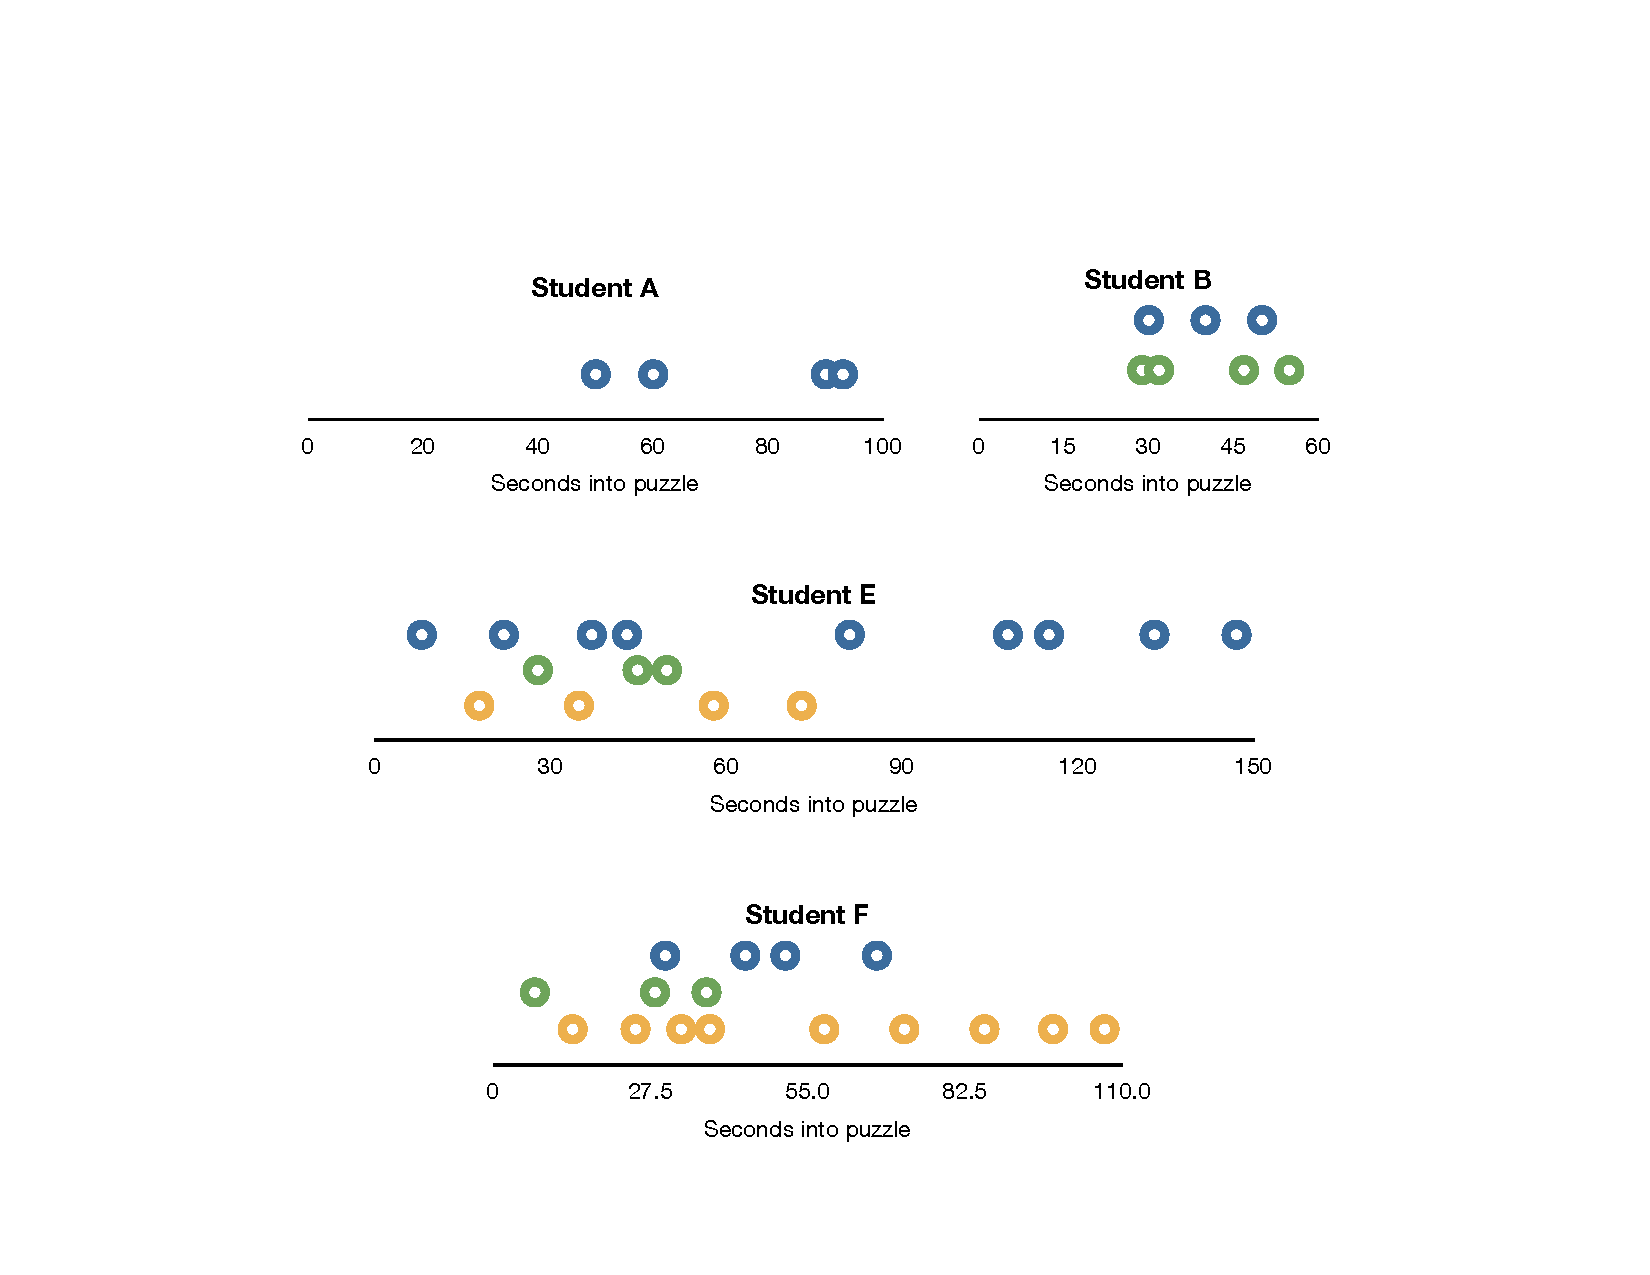
\includegraphics[width=\textwidth]{timelines/rushhour-2.pdf} 
\caption[Rush Hour activity iteration timelines.]{Rush Hour Activity iteration timelines. Each graph represents one student. Each mark represents a test occurring at the specified time. Each row is a different puzzle that the student completed. The horizontal axes are time, in seconds.}
\label{fig:rushhour-timeline}
\end{figure}

Students were observed iterating extremely quickly, often with only seconds between iterations, as seen in Figure~\ref{fig:rushhour-timeline}. Students were unsure about their own processes, and often contradicted themselves when explaining how they developed strategies. Very little process description provided by the students was supported by the observations during the session. 

This game was a good introductory activity because its easiness to learn.

%%%%%%%%%%%%%%%%%%%%%%%%%%%%%%%%%%%%%%%%%%%%%%
%%%%%%%%%%%%%%%%%%%%%%%%%%%%%%%%%%%%%%%%%%%Lights
\section{Light Optimization Analysis}

This activity had a well-defined schedule and a structured metric of design success, which was made explicit to the students in the form of a mathematical calculation. The session was broken into two phases, with each phase containing a complete problem solving cycle. The second phase presented the same problem as the first, but with component price values modified, changing the location of the optimal point in the solution space. Testing was also very deliberate, as it required the use of the power supply. Rules were in place that students could only turn on the power supply when their system was safe and nobody was touching the circuit. Unlike other activities, test feedback could not be generated without the power supply being on, making the test cycles relatively formal.

For students, the metric of design success was based on a formula, and students turned to arithmetic throughout the activity to help them plan and check their designs.

\subsection{Expected and Observed Outcomes}
With two deliberate design phases, it was expected that students would be more successful in the second phase. The first phase was expected be mostly exploration, and the second one was expected to have more frequent iteration and testing cycles. This was shown to be at least superficially accurate, as more iteration cycles occurred across all the students in the later portion of the session. When looking at the entire session as a whole, however, the concentration of iterations was congruent with that of other activities that did not have deliberate phases. It is possible that the increase in testing cycles indicates a greater pattern of developing comfort with the problem over time, and the forced phases may have had little effect. 

%\subsection{Observed Behaviors}

%\subsection{Wrapup Discussion}

\subsection{The 1-Wire Misconception} \label{sec:1wire}
A misconception was observed that was completely unexpected and provided a serious problem for the students experiencing it: thinking power can flow over a single wire. Students with this misconception were unable to build a working circuit until they received additional corrective instruction from the researchers. The students C and D created their first design to look like a lollipop: one wire came from the power supply and connected to one point in a series loop of lights. The other terminal of the power supply went to a similar loop. Clearly this circuit did not function, as there was no circuit created between the two terminals of the power supply. 

\subsection{Voluntary Use of Math} \label{sec:students-math}
The most unexpected and significant observation made during this session was the students voluntarily using written algebra to help their designs. Without any prompting from researchers, students took it upon themselves to manipulate the scoring formula to find how many lights and wires they wanted to strive for to make a certain score. They then revisited that formula after testing to validate their design. While the subjects were above-average students, using mathematics in both planning and validation is usually only observed in designers with engineering training. 

\subsection{Light Optimization Results}

\begin{figure}
\centering
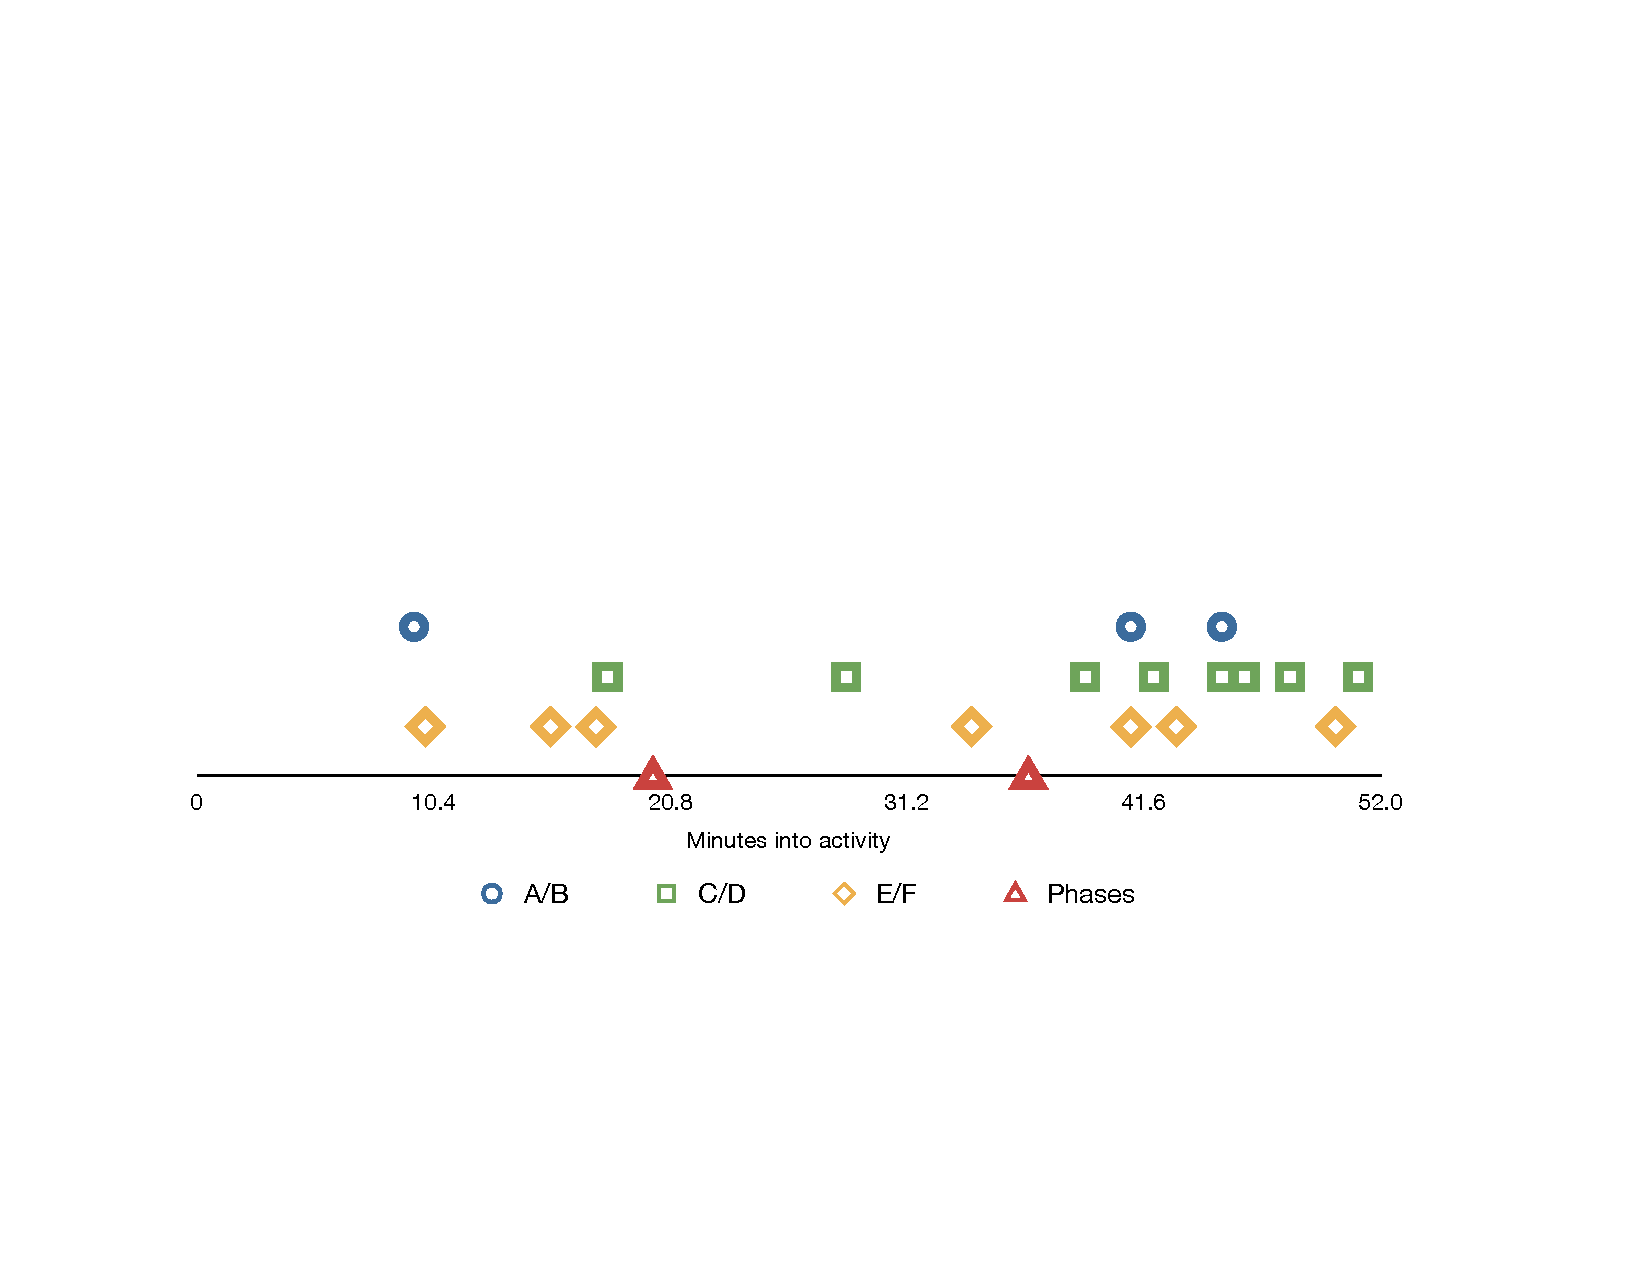
\includegraphics[width=\textwidth]{timelines/lights-2.pdf} 
\caption[Light Optimization activity iteration timeline.]{Light Optimization Activity iteration timeline. Each mark represents a test occurring for the specified student dyad. Each row represents a different student group. The triangular marks indicate the end of the first design phase and the beginning of the second. The horizontal axis is time, in minutes.}
\label{fig:lights-timeline}
\end{figure}

Figure~\ref{fig:lights-timeline} shows a timeline of all iterations performed by students during this activity. The first design phase ended at 20 minutes, and is marked by the first triangle on the timeline. The second phase, with modified design criteria, began at 36 minutes, and is indicated by the second triangle. In the time between the two phases, students analyzed their first design and prepared for their second. Two groups performed tests during this period, as can be seen in the figure. Additionally, this figure shows that the second design phase contained many more iterations than that first for all groups. 

This activity was included for numerical analysis. Table~\ref{tab:results-lights} shows that the most successful student group (A/B) had the fewest number of iterations. This dyad utilized prior knowledge to deliver a working design on the first try and were satisfied with that design for the remainder of the session. That student pair recognized the holiday lights and immediately recalled how a string of Christmas tree lights work. They proceeded to build a series string, like that of the Christmas tree, and had a working solution very quickly. The second phase of the activity forced a redesign by changing the parts costs, but group A/B determined their solution also satisfied the revised requirements, and they left their design essentially unchanged. 

Putting aside the above dyad, the other two groups (C/D and E/F) were fairly similar in iteration count, average iteration time, and non-iterating introductory time. The biggest difference between them was that group~C/D spent more time in introduction before beginning testing. Group~C/D had the 1-wire misconception of electricity which gave them a disadvantage, as discussed in Section~\ref{sec:1wire}. Both of these groups met the first level of success. 

The most significant observation was the students' self-motivation to use mathematics to improve their design, discussed in Section~\ref{sec:students-math}.

\begin{table}
\begin{centering}
\begin{tabular}{l c c c}
	%\multicolumn{4}{l}{{\large Elevator Control Specifications}} \\
	\toprule
					& A/B 	& C/D 	& E/F 	\\ \midrule
	Iteration Count          & 3 		& 8 		& 7		\\ \midrule
	Time per iteration 	& 18 min	& 5 min	& 7 min	\\ \midrule
	St.Dev. of time per iteration 	& 14.8 min & 3.7 min & 4.8 min \\ \midrule
	Non-iterating time 	& 21\%      & 35\%	& 20\% 	\\ \midrule
	Success (0,1,2)	& 2		& 1		& 1		\\ 
	\bottomrule
\end{tabular}
\caption[Results from the Light Optimization activity.]{Results from the Light Optimization activity. The best performing team had the fewest iterations, which is believed to be based on that team utilizing prior knowledge.}
\label{tab:results-lights}
\end{centering}
\end{table}

%	\begin{figure}[htbp]
%	\begin{center}
%	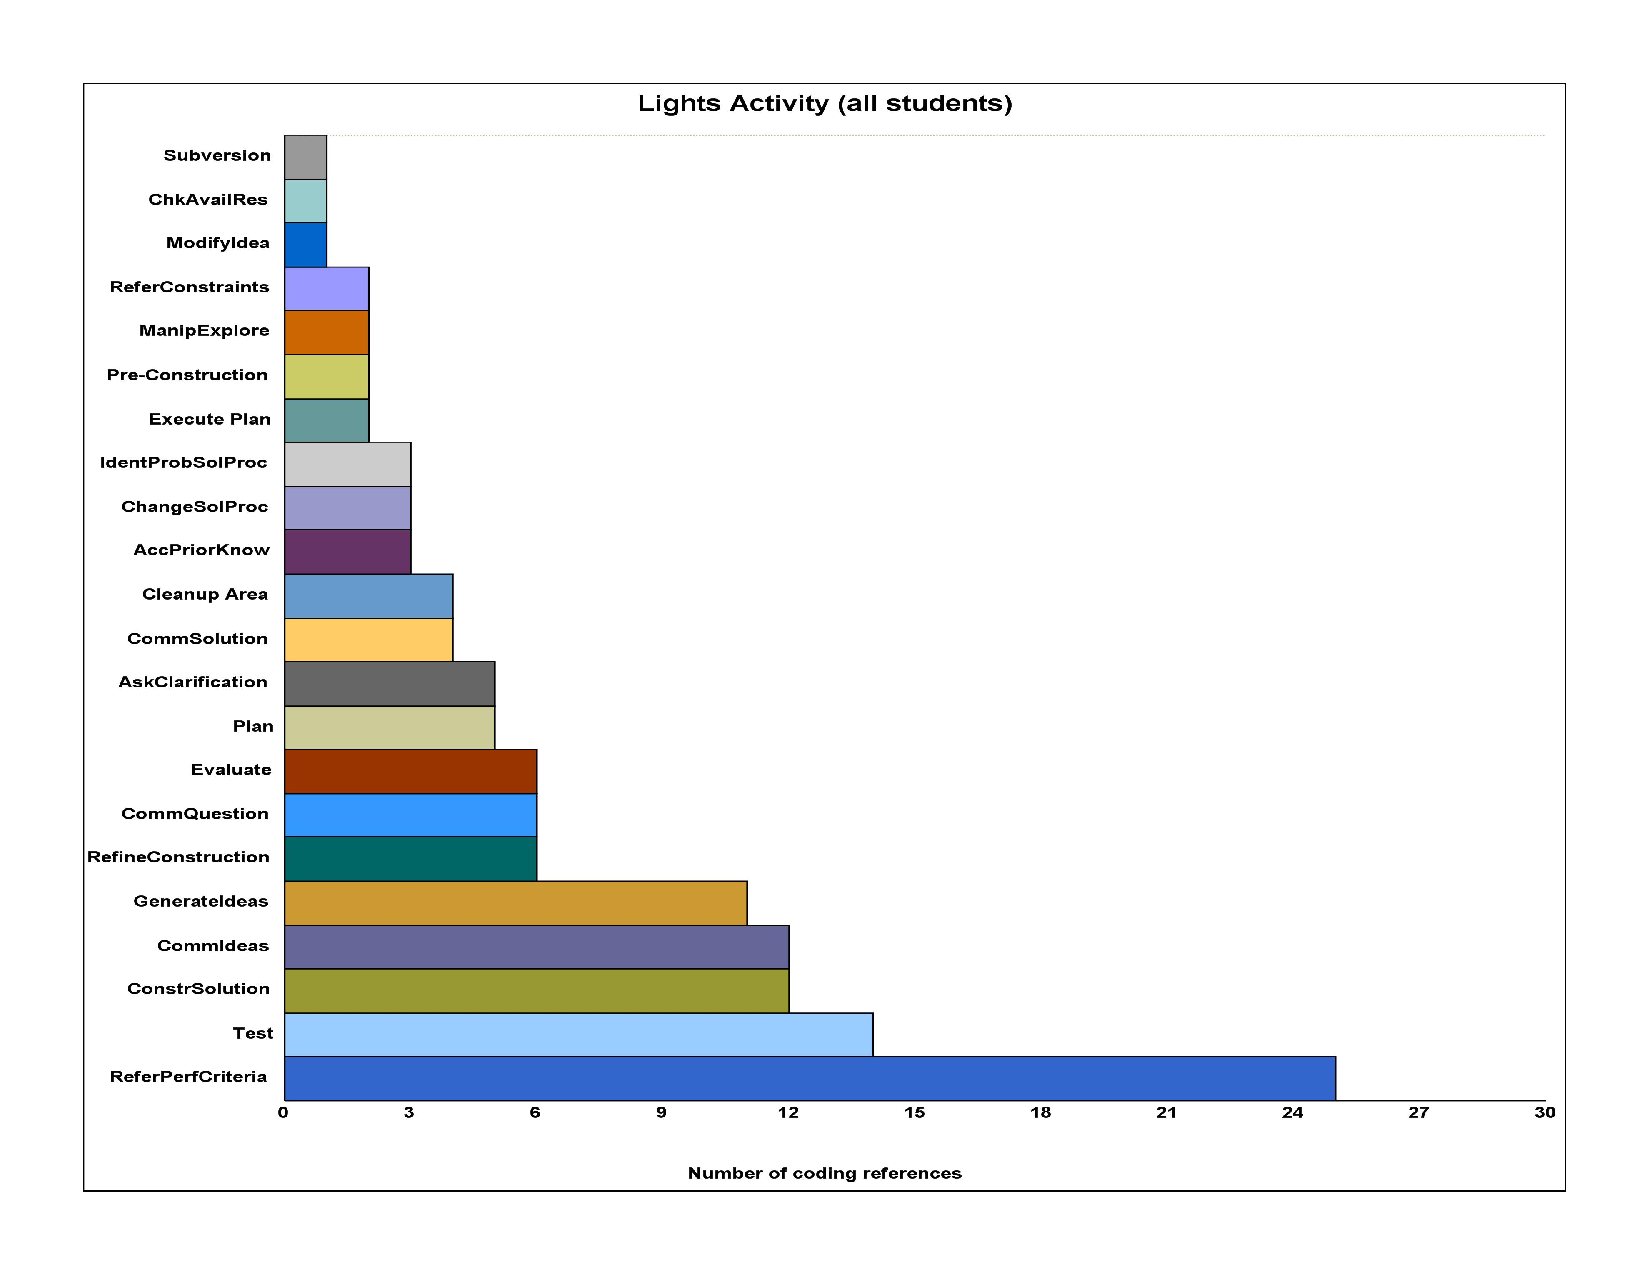
\includegraphics[width=\textwidth, height=\textwidth]{charts/lights1-code-count.pdf}
%	\caption{Number of coding references for all students during the Lights activity.}
%	\label{fig:lights-code-count}
%	\end{center}
%	\end{figure}

%%%%%%%%%%%%%%%%%%%%%%%%%%%%%%%%%%%%%%%%%%%%%%
%%%%%%%%%%%%%%%%%%%%%%%%%%%%%%%%%%%%%%%%%%%Gears
\section{Gear Reduction Activity}

\begin{figure}
\centering
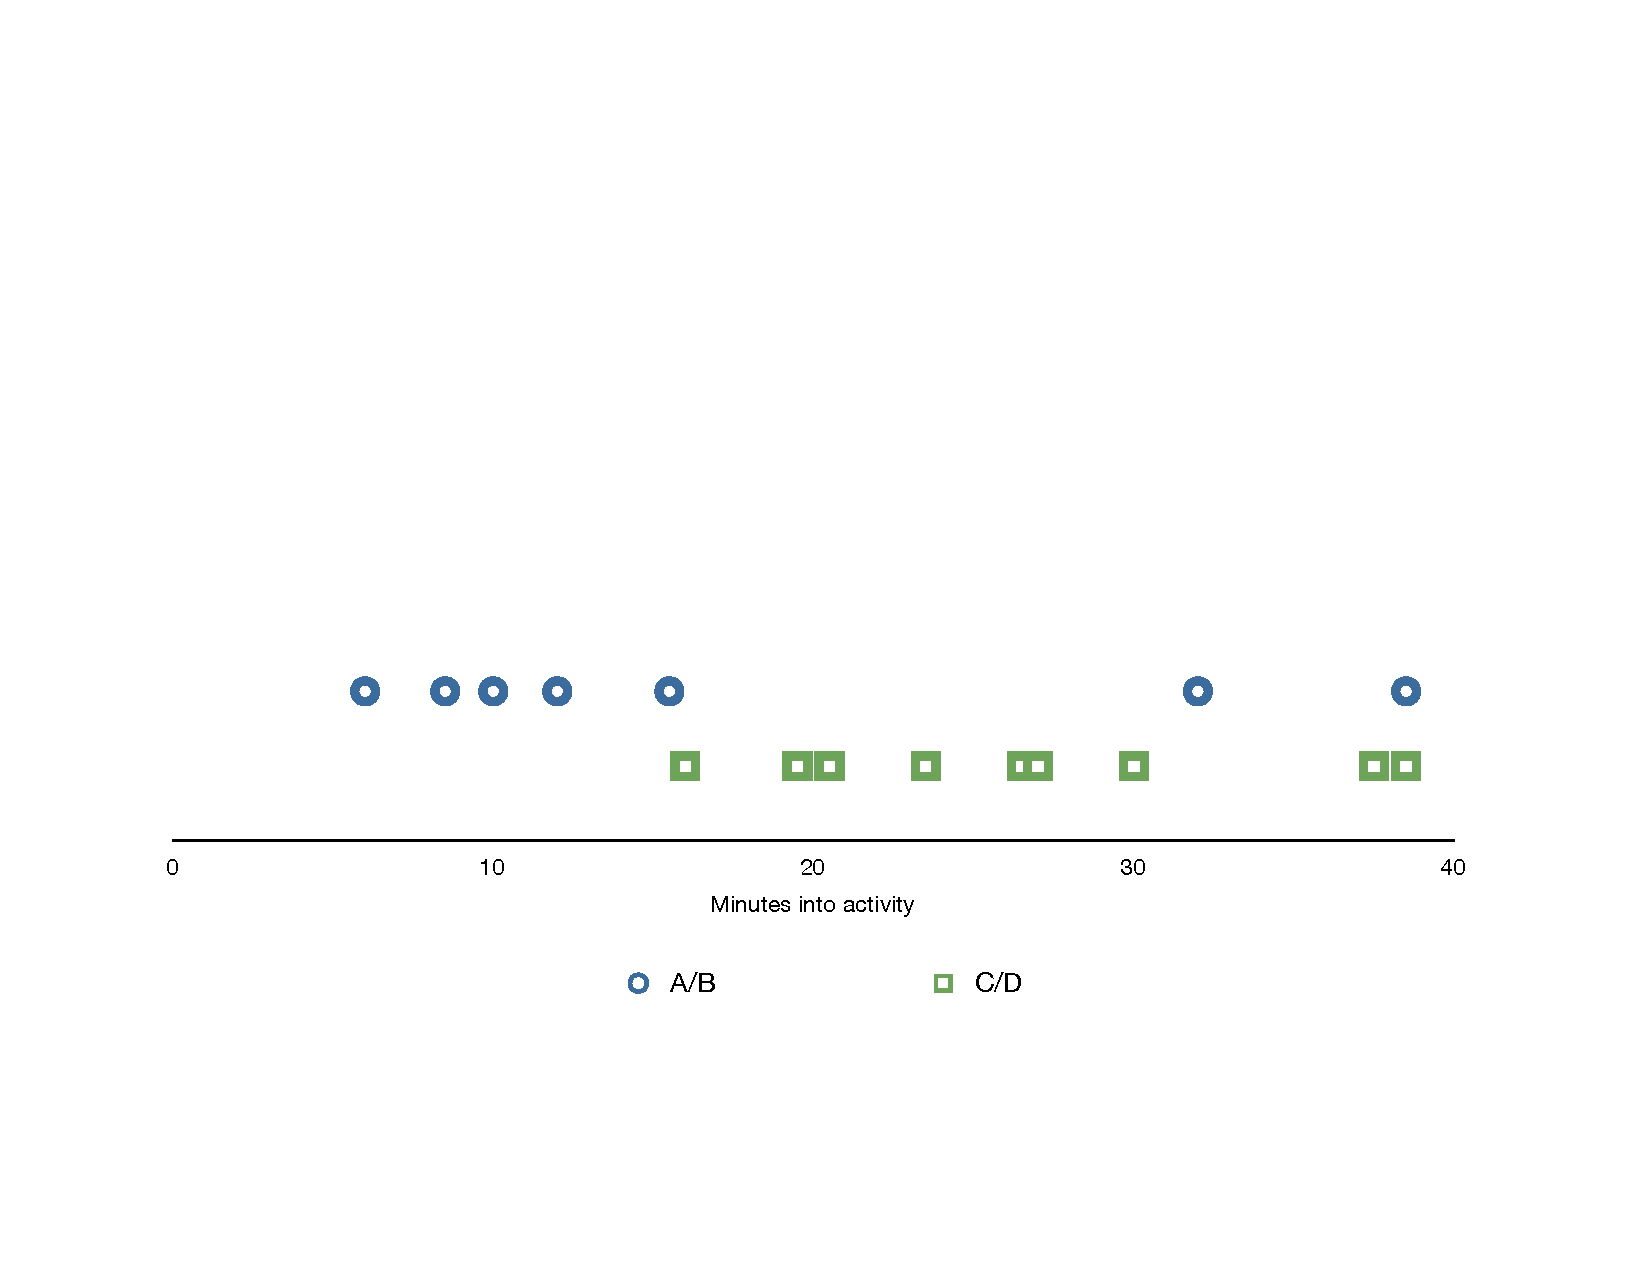
\includegraphics[width=\textwidth]{timelines/gears-2.pdf} 
\caption[Gear Reduction activity iteration timeline.]{Gear Reduction activity iteration timeline. Each mark represents a test occurring for the specified student dyad. Each row represents a different student group. The horizontal axis is time, in minutes.}
\label{fig:gears-timeline}
\end{figure}

The Gear Reduction activity had the students build LEGO structures that enable a small motor to lift a mass via gear reduction. This activity is complex, and required not just an understanding of gear reduction, but of LEGO construction as well. This proved to be a harder problem than anticipated by the researchers.

\subsection{Expected and Observed Outcomes}
This activity was intended to be an exercise in gear spacing, meshing, and reduction. Students were expected to choose testing patterns somewhere on the continuum between large numbers of small, local tests and small number of large, entire-system tests. The best solutions were expected to come from students who iterated more often. This hypothesis was demonstrated to be generally correct, but was complicated by the unexpected degree of difficulty of the activity. 

\subsection{Difficulty in Construction}
In the other activities presented in this project, the students were designing against a highly constrained physical world (the Light Optimization activity), a simulated, abstract environment (the Elevator Control activity), or used a symbolic world (the ``Rush Hour" and Word Search activities). In the Gear Reduction activity, the student design was tested directly against nature, which provided many unanticipated complications. The challenge was not focused on gear ratios as expected, but on the more general and difficult task of building. Students were plagued with an under constrained design space including part selection, structure design, gear choice, and component connections. Despite the unexpected difficulty, most students (two of the three dyads) did succeed in solving the design problem. However, the process-oriented model that was desirable was lost as students focused entirely on finding a single working solution.

%\subsection{Observed Behaviors}
%\subsection{Wrapup Discussion}
\begin{table}
\begin{centering}
\begin{tabular}{l c c c}
	\toprule
					& A/B 	& C/D 	& E/F 	\\ \midrule
	Iteration Count          & 7 		& 8 		& 0		\\ \midrule
	Time per iteration 	& 5 min	& 3 min	& 		\\ \midrule
	St.Dev. of time per iteration 	& 4.8 min & 2.1 min & \\ \midrule
	Non-iterating time 	& 15\%      & 42\%	& 100\% 	\\ \midrule
	Success (0,1,2)	& 1		& 2		& 0		\\ 
	\bottomrule
\end{tabular}
\caption[Results from the Gear Reduction activity.]{Results from the Gear Reduction activity. The best performing team had the longest non-iterating time, with the exception of group~E/F, who never advanced to testing.}
\label{tab:results-gears}
\end{centering}
\end{table}

\subsection{Gear Reduction Results}

The iterations performed by the students in this activity are shown on a single timeline in Figure~\ref{fig:gears-timeline}. The two groups shown had very different iteration patterns. Group~A/B is bimodal, with many iterations in the beginning and end segments of the activity. Group~C/D started iterating later in the session, and was more consistent with iteration spacing. Group~E/F did not perform any iterations. All of these observations are analyzed in detail below.



This activity was included for numerical analysis. The results are shown in Table~\ref{tab:results-gears}. Dyad~E/F never advanced to performing a test, and as such is listed with zero iterations and a non-iterating time of 100\%. This group did not successfully complete the activity. Excluding that pair, the most successful student group, C/D, had the longest introductory time at 42\%. Group~A/B had nearly the same number of iterations as C/D, but they were more spread out over the session time. C/D iterated faster, with more consistent time per iteration. Both A/B and C/D achieved successful solutions, but only C/D achieved a generalized process.

Building with LEGO is difficult. This activity was more difficult than expected and did not carry the intended focus of pure gear mechanics. The groups who managed to perform tests and iterations did overcome these problems, and the group that did not test did not achieve any levels of success.

\begin{figure}
	\begin{centering}
	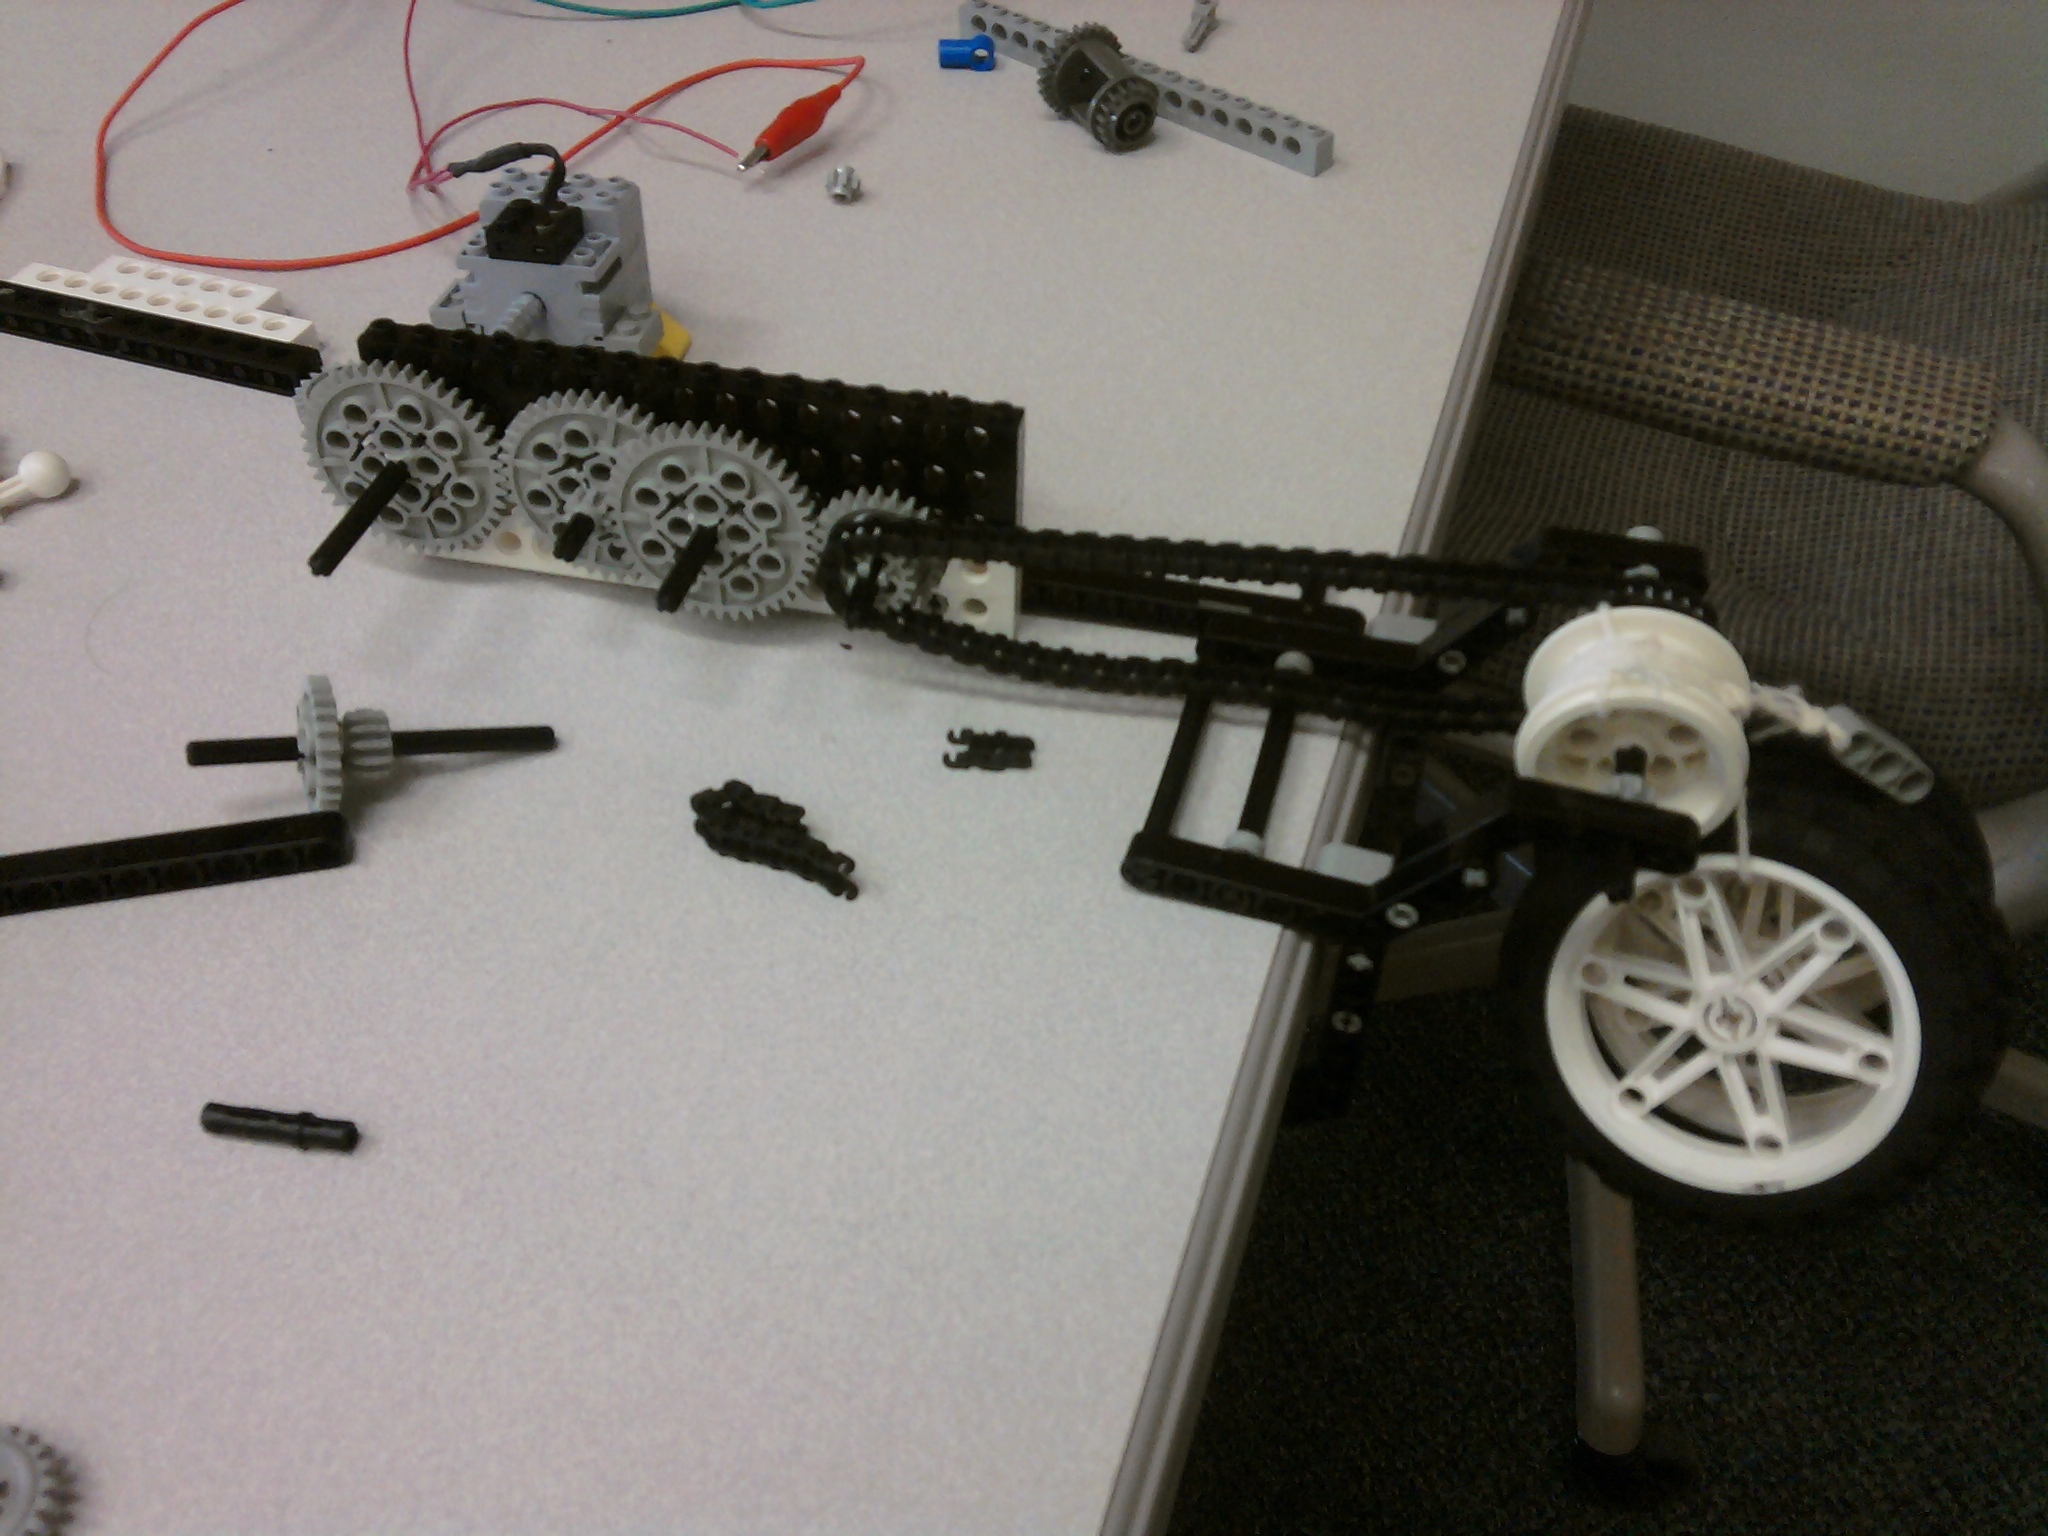
\includegraphics[width=\textwidth]{product/gears-1}
	\end{centering}
	\caption[Gear Reduction solution made by C/D dyad.]{Gear Reduction solution made by C/D dyad. This design successfully completed the task. This image includes the mass that was lifted, which are the large wheels to the right.}
	\label{fig:gearsCD}
\end{figure}

\begin{figure}
	\begin{centering}
	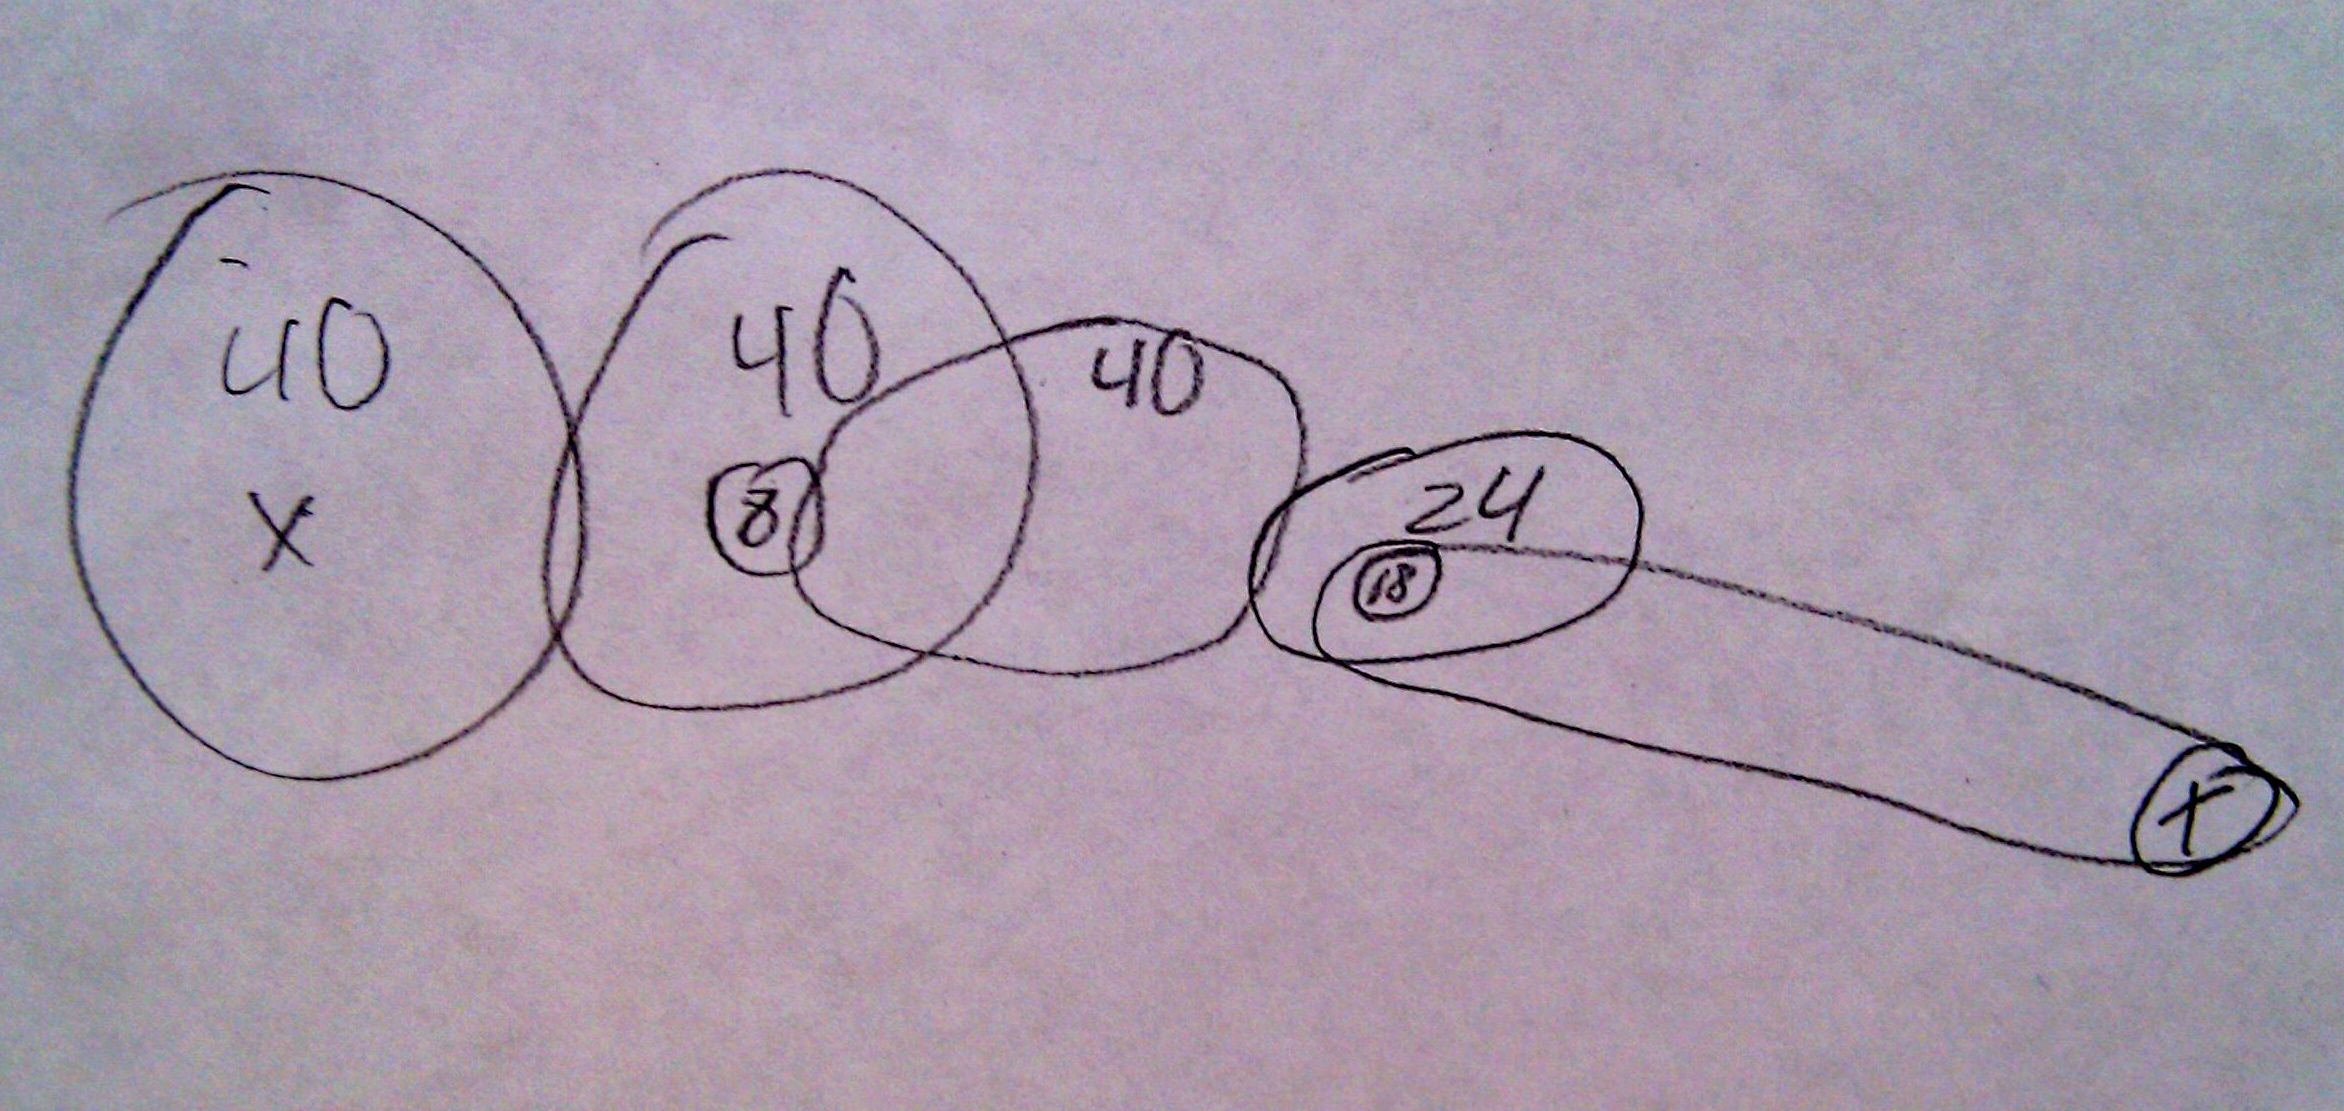
\includegraphics[width=\textwidth]{product/sp-gear-2}
	\end{centering}
	\caption{Gear Reduction Solution diagram by C/D dyad. }
	\label{fig:gearsCD-dia}
\end{figure}

The solution built by group~C/D scored the highest success rating, and is shown in Figure~\ref{fig:gearsCD}. The diagram they drew is seen in Figure~\ref{fig:gearsCD-dia}. This group had one stage that actually performed a reduction of 8:40. The design included an unnecessary 1:1 stage and a counter-productive 40:24 gear increase. The overall reduction was sufficient to complete the task, and the construction was solid.

\begin{figure}
	\begin{centering}
	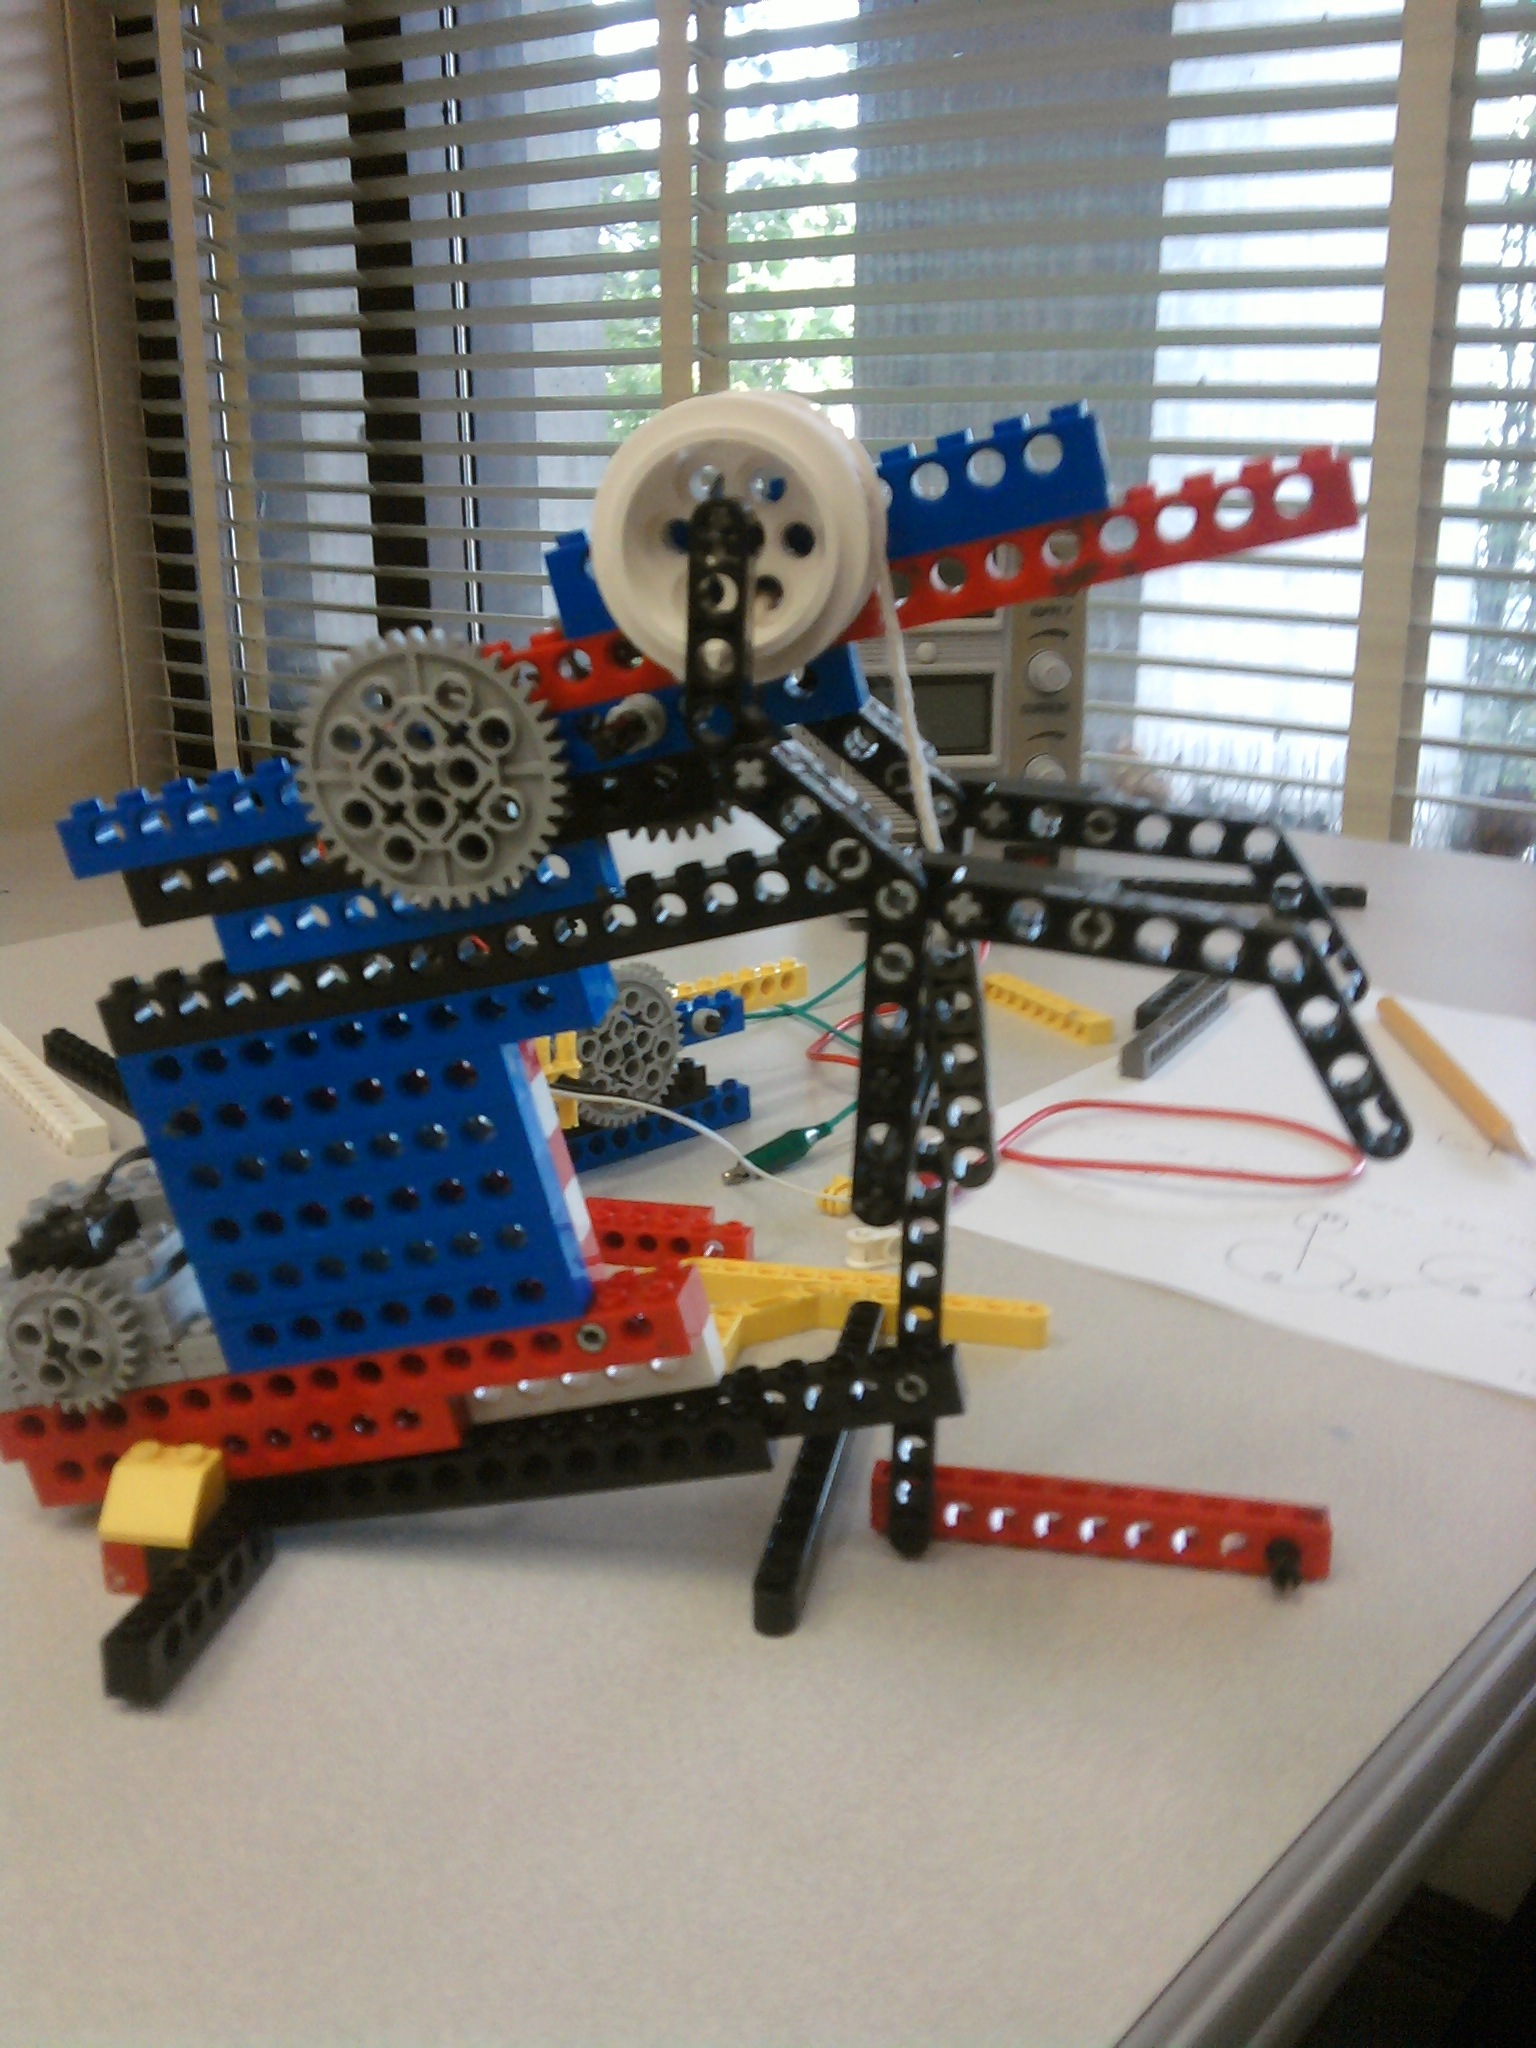
\includegraphics[width=\textwidth]{product/gears-3}
	\end{centering}
	\caption[Gear Reduction solution made by A/B dyad, front view.]{Gear Reduction solution made by A/B dyad, front view. This design was successful, but not as solid as the one made by C/D. A length of chain is called for to connect the motor at the far left to the large gear in the center (not shown).}
	\label{fig:gearsABfront}
\end{figure}
	
\begin{figure}
	\begin{centering}
	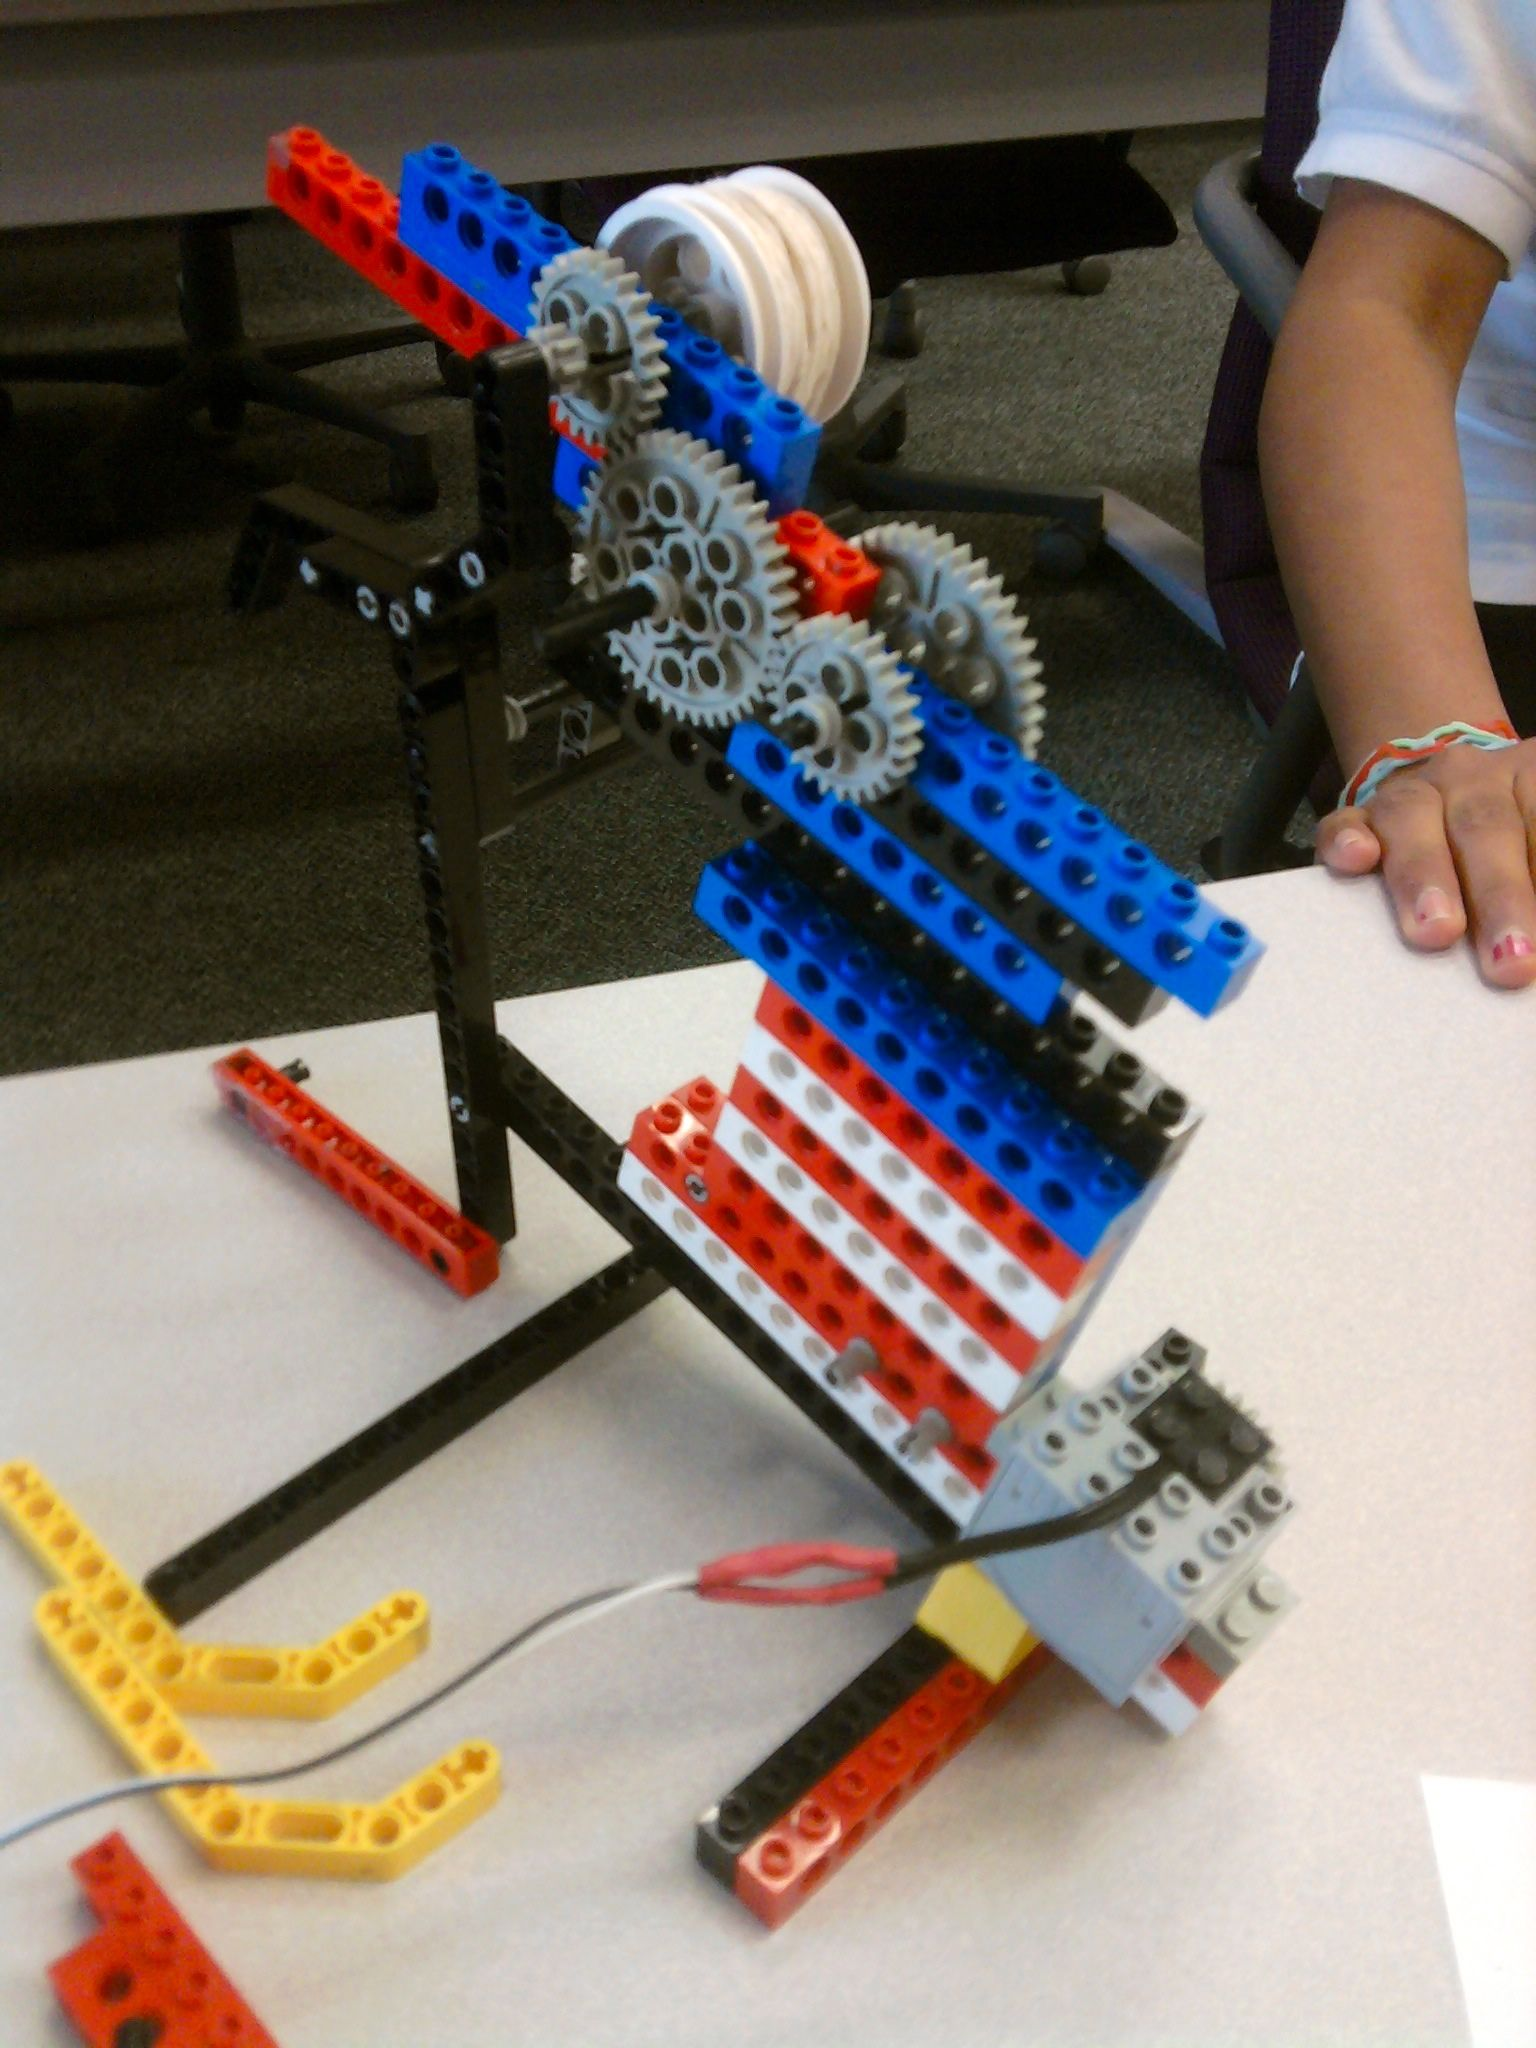
\includegraphics[width=\textwidth]{product/gears-4}
	\end{centering}
	\caption{Gear Reduction solution made by A/B dyad, rear view.}
	\label{fig:gearsABback}
\end{figure}

The solution built by group~A/B is shown in Figures~\ref{fig:gearsABfront} and~\ref{fig:gearsABback}, with their diagram shown in Figure~\ref{fig:gearsAB-dia}. The design was theoretically sound, employing three stages of 24:40 reduction. The construction was weak, but sufficient to survive the one-day activity.

\begin{figure}
	\begin{centering}
	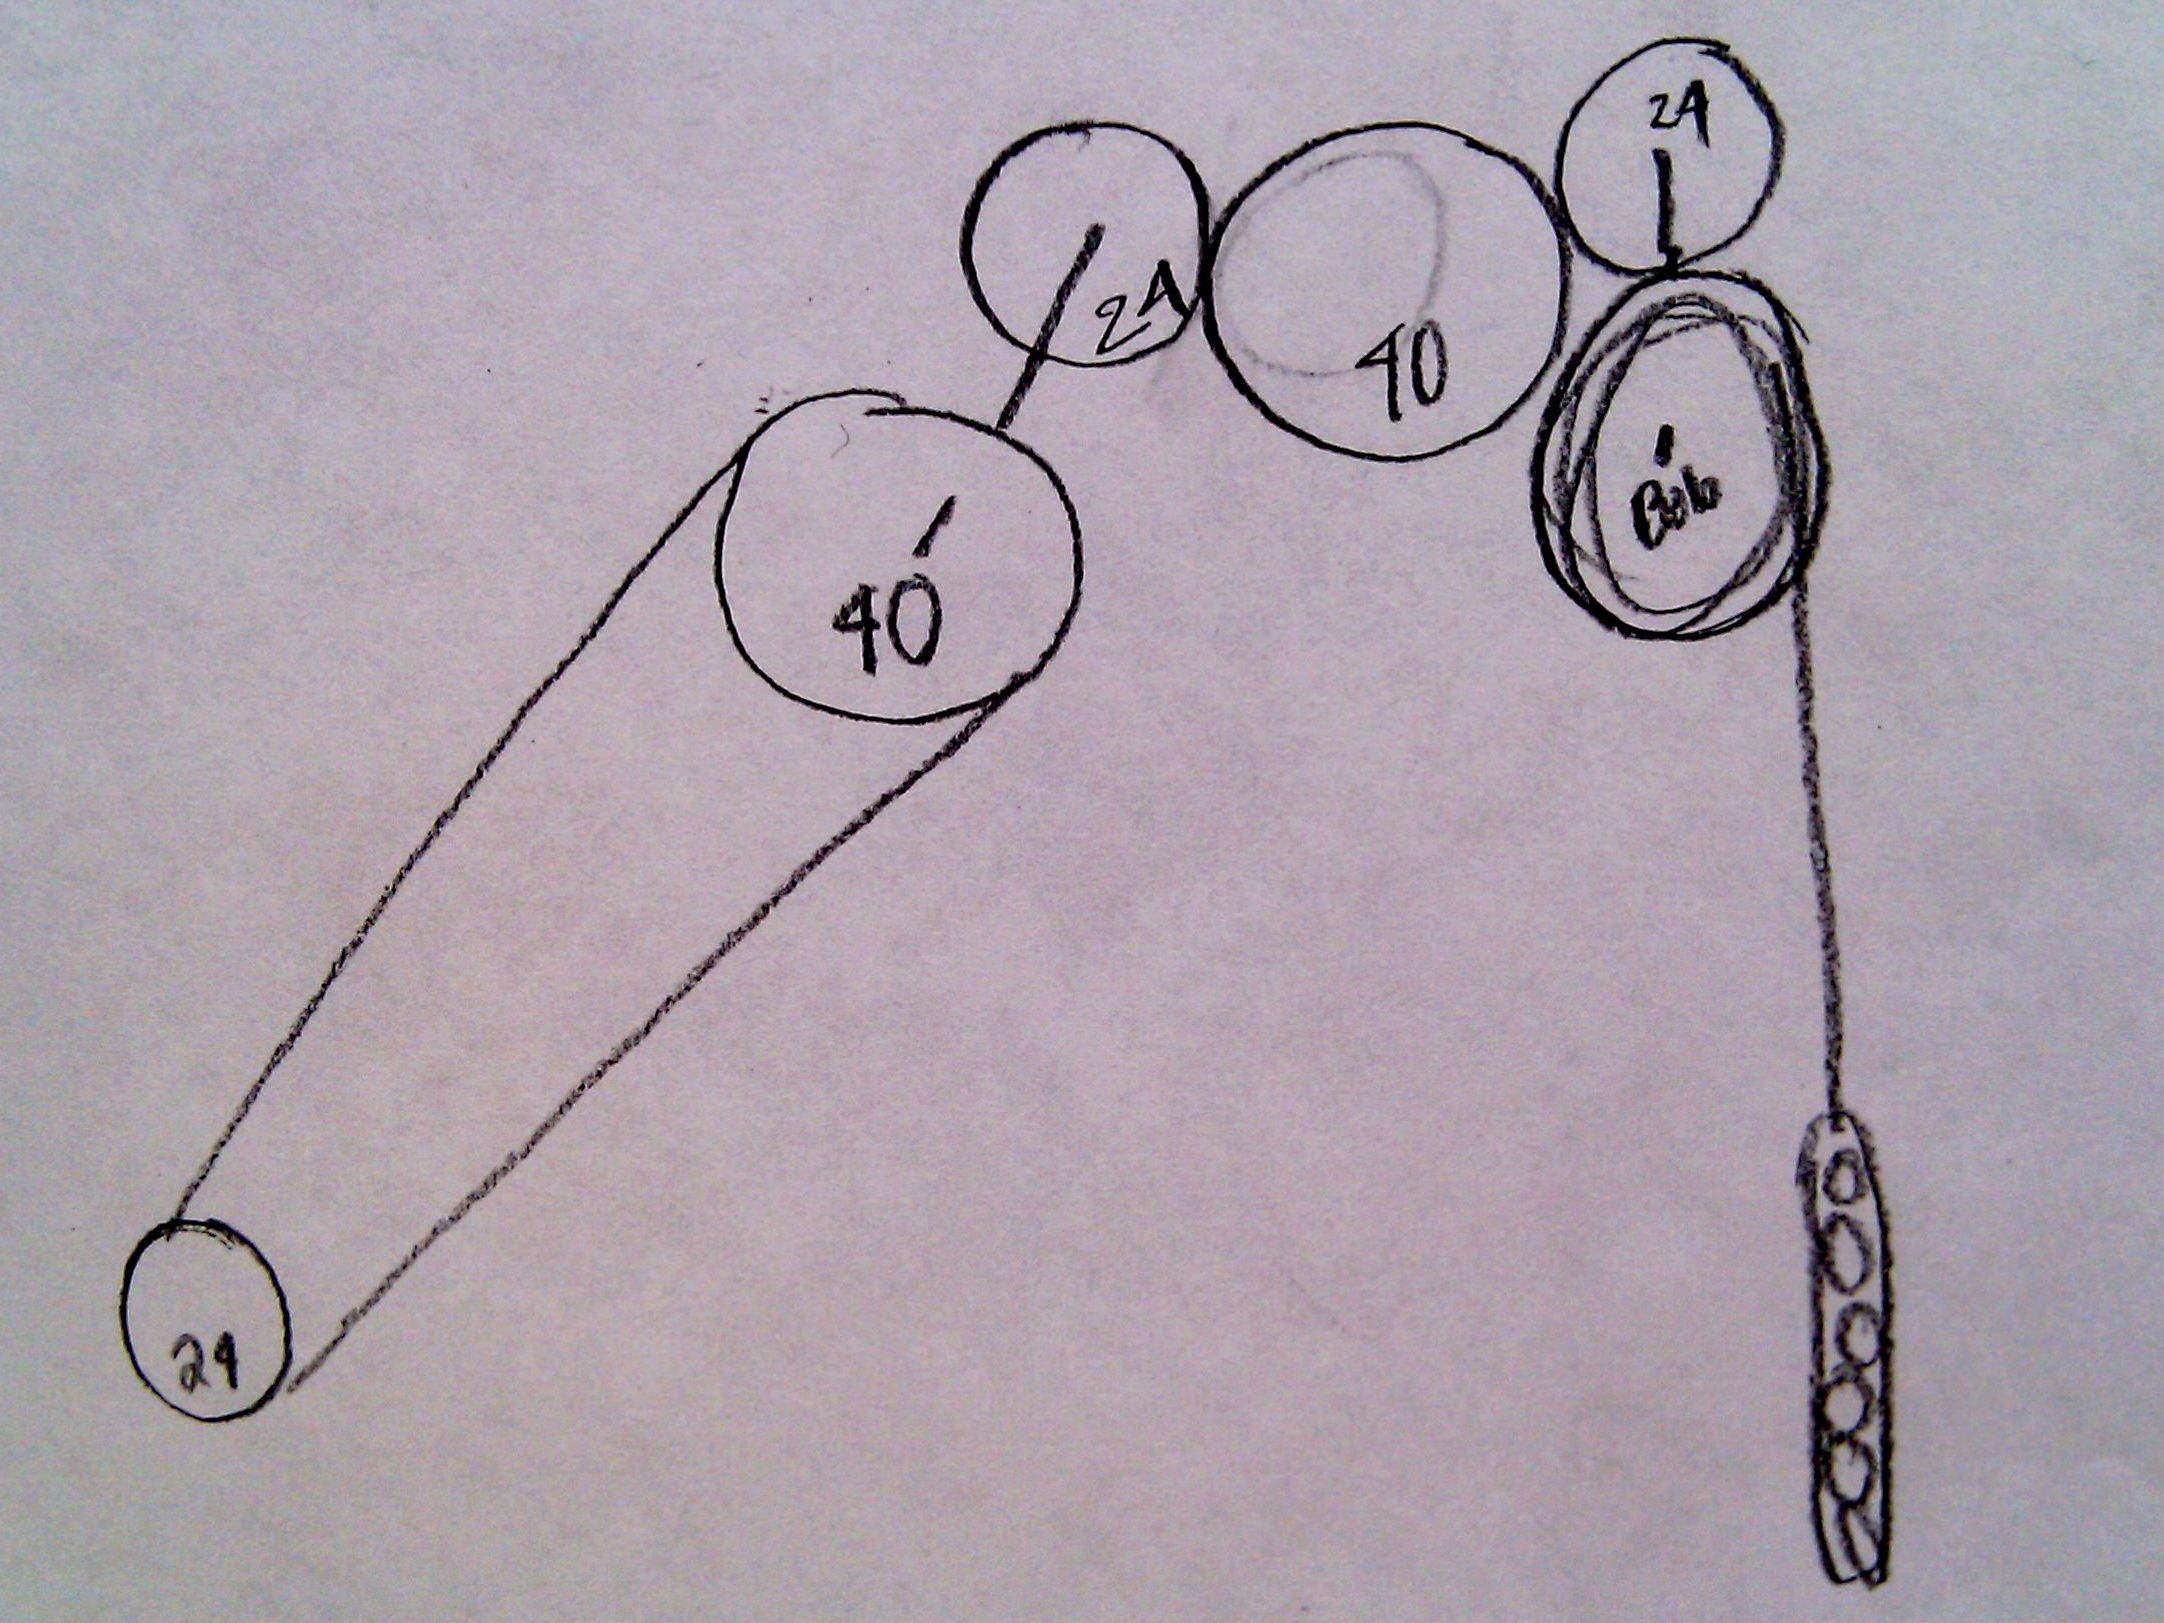
\includegraphics[width=\textwidth]{product/sp-gear-4}
	\end{centering}
	\caption{Gear Reduction solution diagram by A/B dyad. }
	\label{fig:gearsAB-dia}
\end{figure}

\begin{figure}
	\begin{centering}
	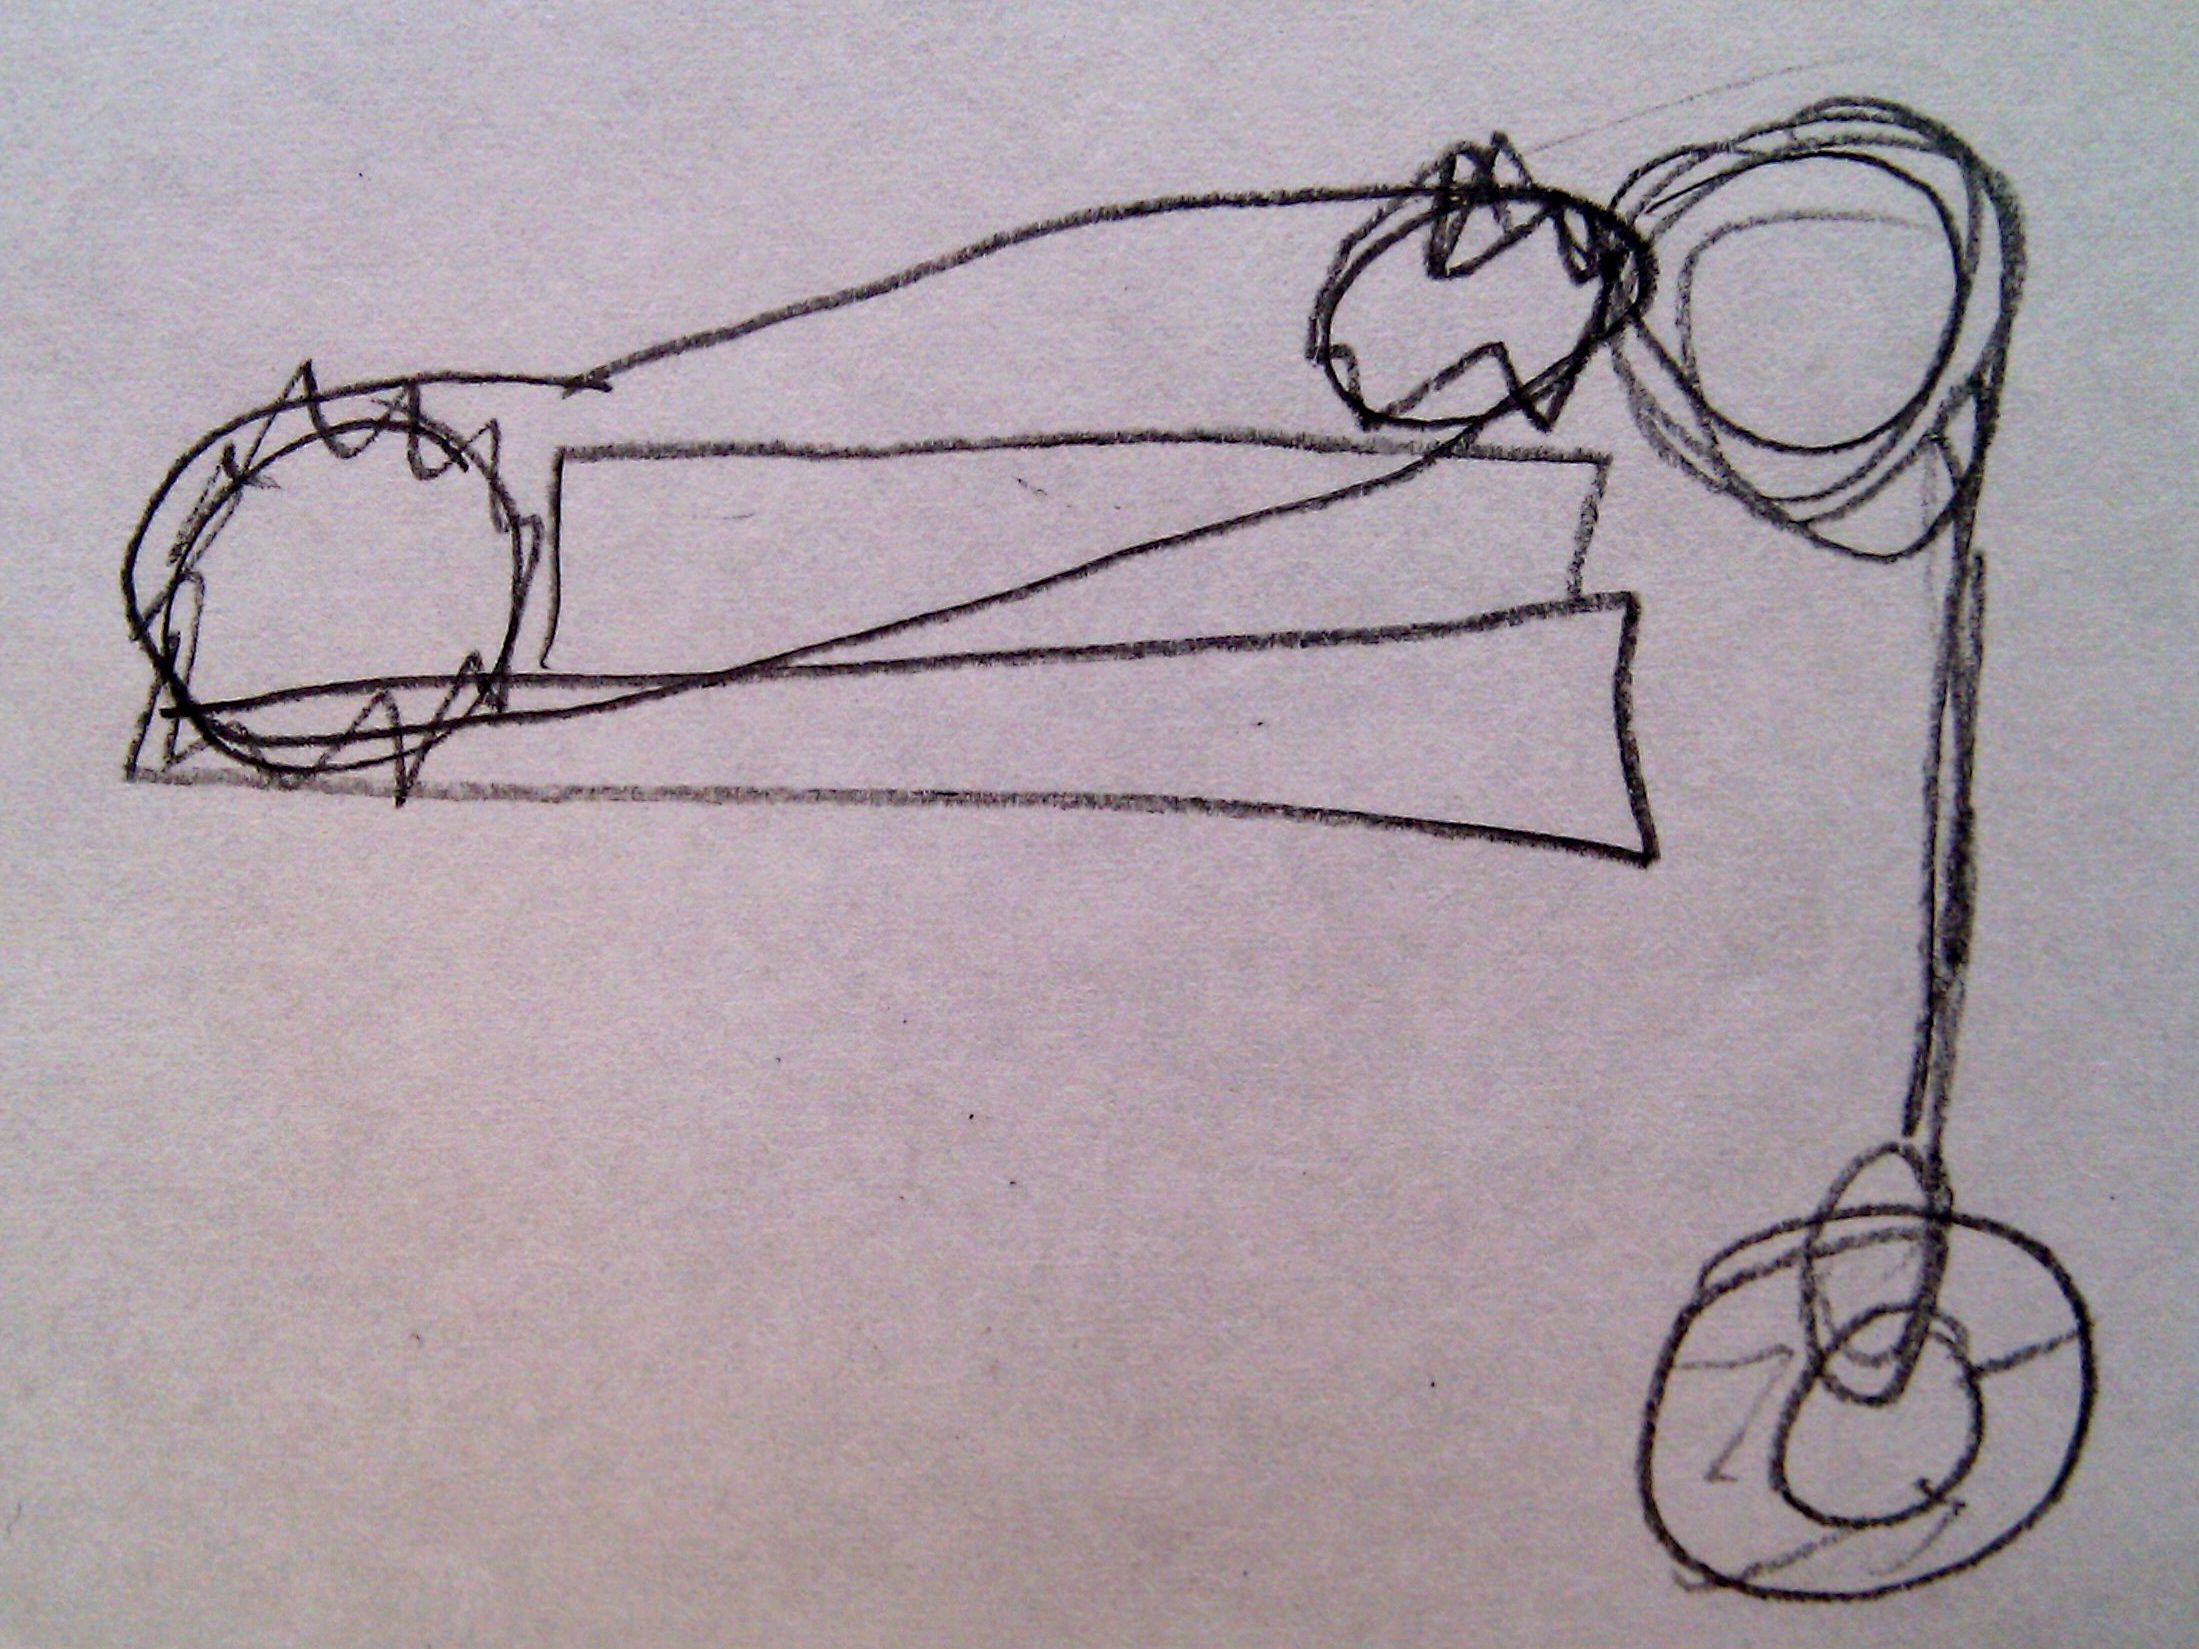
\includegraphics[width=\textwidth]{product/sp-gear-1}
	\end{centering}
	\caption[Gear Reduction solution diagram by E/F dyad.]{Gear Reduction solution diagram by E/F dyad. This group never tested their design, nor came to a working solution. The diagram lacks detail of the system. }
	\label{fig:gearsEF-dia}
\end{figure}

The group that did not complete, group~E/F, provided a diagram that is shown in Figure~\ref{fig:gearsEF-dia}. This diagram lacks detail of the gear interactions. It does not specify any gear sizes, nor does it indicate how the gears actually connect together. The diagram is an abstract representation of a the general shape of a solution, but does not specify any actual implementation.

%%%%%%%%%%%%%%%%%%%%%%%%%%%%%%%%%%%%%%%%%%%%%%
%%%%%%%%%%%%%%%%%%%%%%%%%%%%%%%%%%%%%%%%Word Search
\section{Word Search Activity}
	\label{sec:analysis-wordsearch}
	
This activity was designed to be easy for the students to engage with, as most of them were very familiar with word searches. It also provided a good introduction to algorithms, where students could easily see the application of a mechanical process on the word search grid.
	
\subsection{Expected and Observed Outcomes}
The word search was expected to be easy for the students to gain traction with, enabling them to focus on the algorithm design component. The students were expected to have a few test iterations as they worked through how algorithms function. The activity itself was relatively simple; it was so simple that many students lost interest before the end of the session. In practice though, this session was successful. Students maintained engagement for the majority of the period and held to the rules of the activity to facilitate the desired learning experience. Half of the students actually created legitimate algorithms; the other half created short lists of human-targeted instructions, and did not break them out to component operations. 

The algorithms the students wrote were classified into one of two categories based on the style of instructions that were used: high-level and low-level. High-level instructions required intelligent interpretation, such as ``look for any letters in the word." Low-level instructions were more basic, and could feasibly be implemented in a machine language, such as ``scan this row for letter \emph{x}." The students were not instructed in this difference; the categories were only for purposes of analysis.


%\subsection{Observed Behaviors}
%\subsection{Wrapup Discussion}

\subsection{Word Search Results}
Students became aware of the concept of an algorithm and understood that they were designing them. This is indicative that students of this age possess the cognitive development to think abstractly at the level that is required for algorithm design. 

Despite the students' understanding of the problem and high level of engagement, the iteration count was low. Most students only performed two significant changes on their algorithms, and these occurred only as artifacts of the session instructions. Most students made these iterations at about 20 and 30 minutes into the activity. One student made one additional iteration at about 40 minutes.

Analysis of this activity is based on the type of instructions the students wrote. High-order instructions were clearly intended to be interpreted by humans, as they required complex reasoning to be executed, such as ``wait for words to pop out." The minority of students used simpler instructions that could be argued as machine-compatible. Simpler instructions included ``look for the first letter" and ``see if second letter is touching it." These simple instructions could be combined to create the behaviors that the majority of students represented in a single statement.
%TODO did this turn into discussion?

An example of high-level instructions can be seen in Figure~\ref{fig:sp-ws-2}. That student wrote an instruction to find the first three letters of the word at once. The statement was very compact, including a built-in exception: ``unless two words have the same 3 letters." This phrasing requires a complex interpretation in order to execute. 

	\begin{figure}
	\centering
	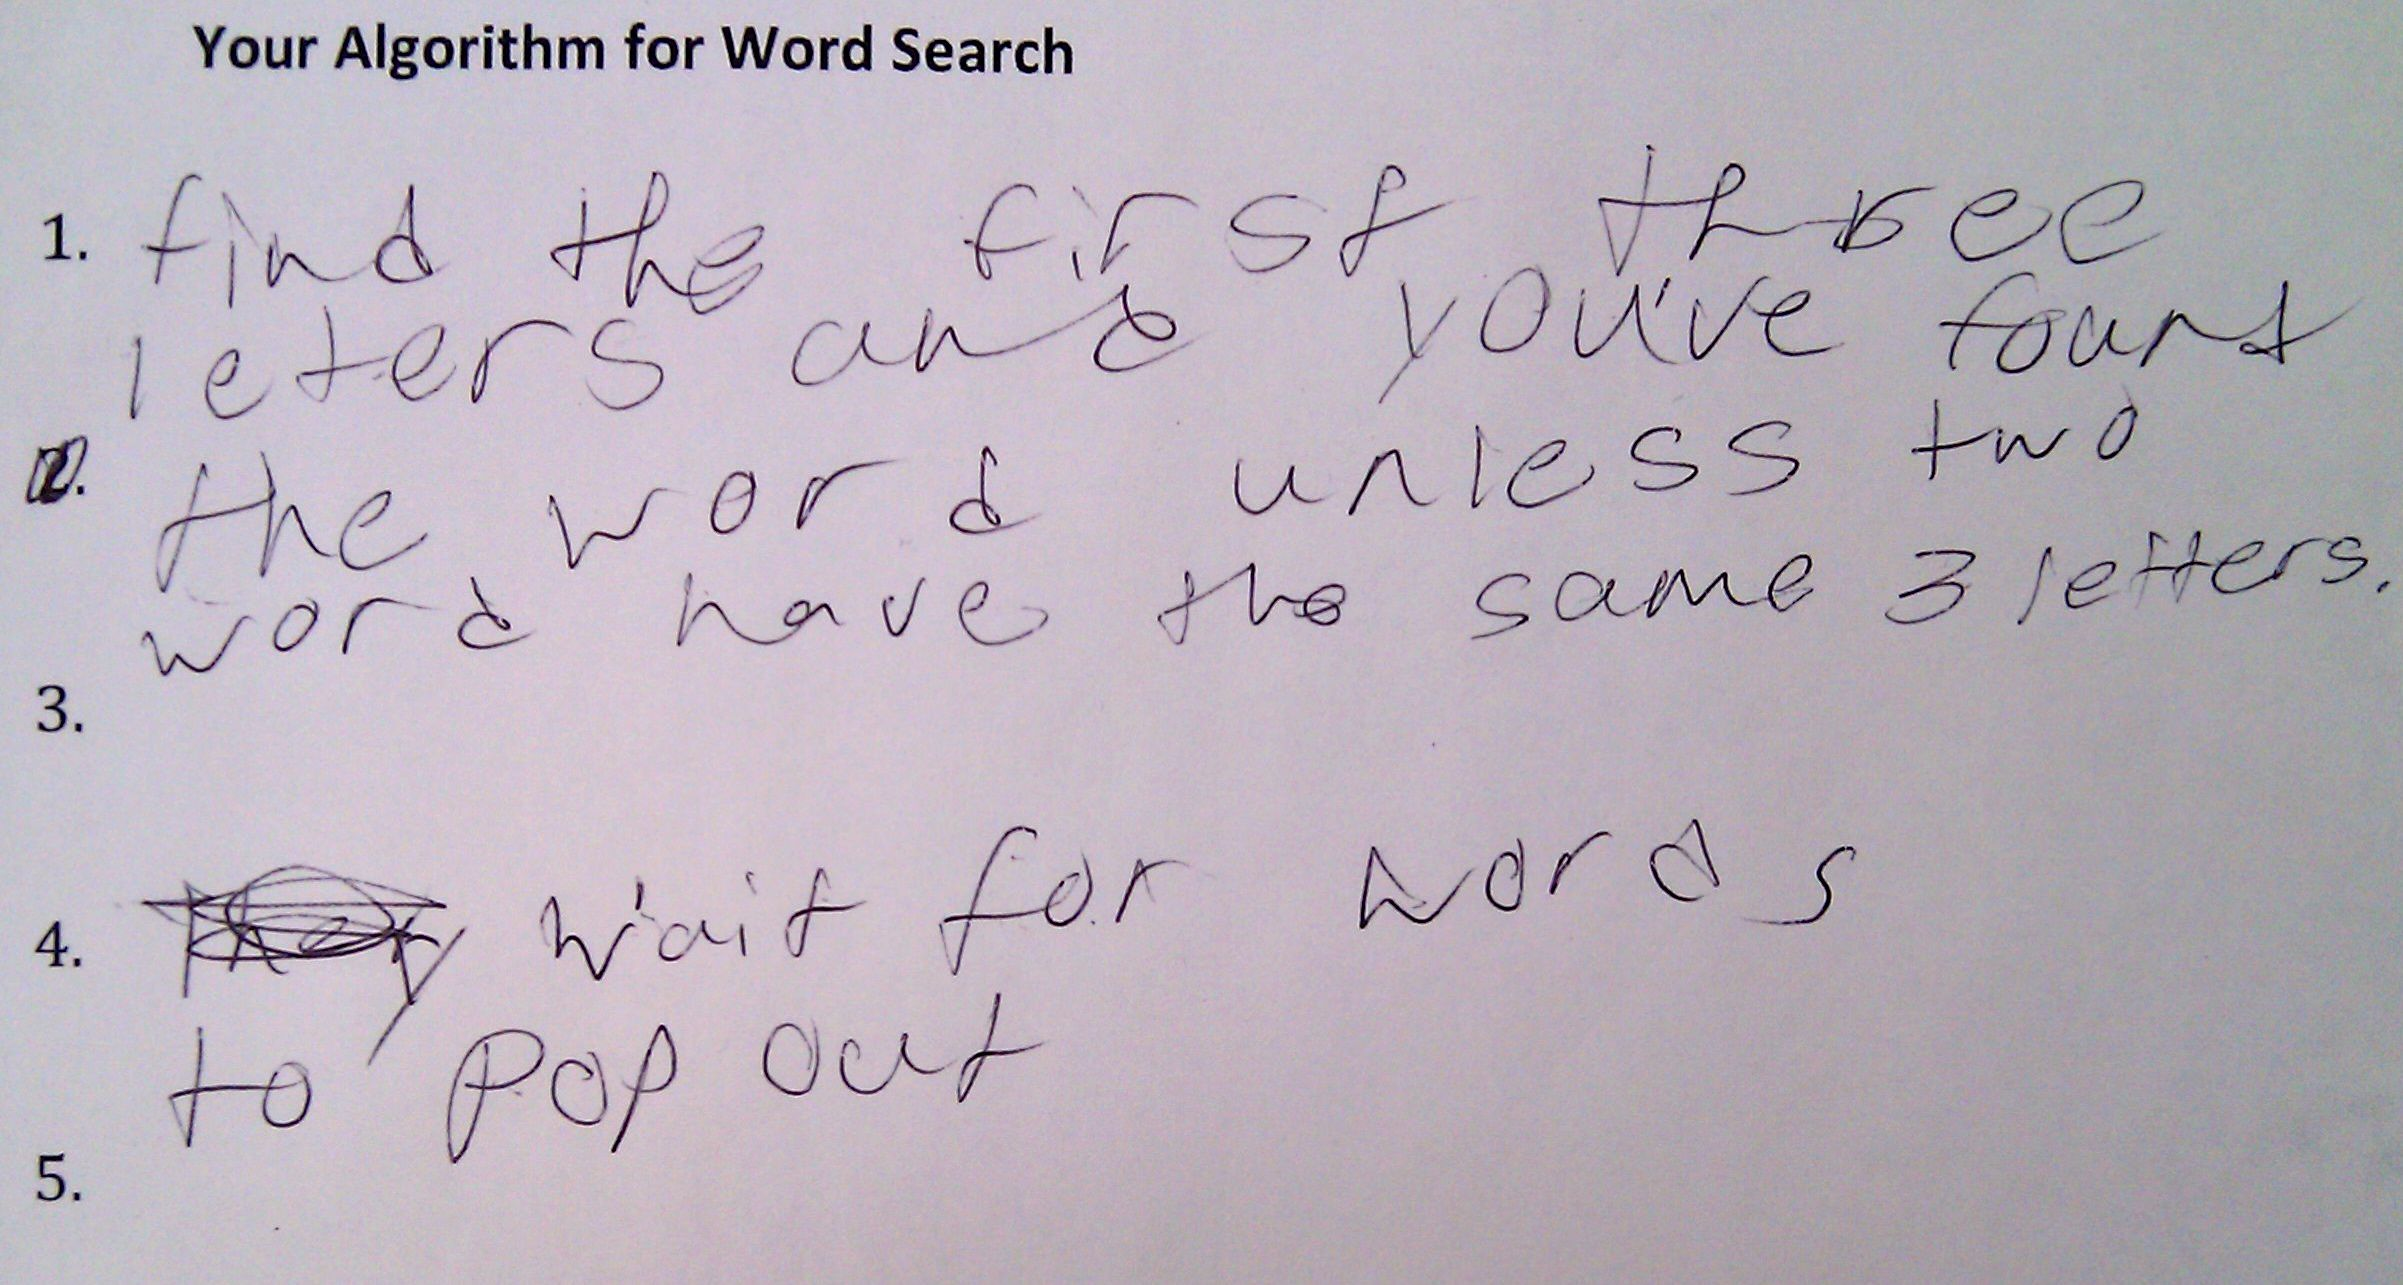
\includegraphics[width=\textwidth]{product/sp-ws-2}
	\caption[Example of a student's algorithm for the Word Search activity.]{Example of a student's algorithm for the Word Search activity. This algorithm uses high-order instructions intended for a human.}
	\label{fig:sp-ws-2}
	\end{figure}

An example of simpler instructions can be seen in Figure~\ref{fig:sp-ws-6}. This student started off in step one with a strategy of ``If you can't find it the first time, try again." This first instruction could be argued to be specifying a loop, which, according to the student's explanation, was the basic intention. Step two is precise, instructing the executor to find the first letter of a word, and then see if the second letter is adjacent. If the second letter is adjacent, check to see if the whole world is there. This step could be broken into to four individual instructions. 

The students who wrote low-level instructions averaged one additional iteration than those who wrote high-level instructions. This could be indicative to additional complexity being required to write a longer series of simpler instructions.

	\begin{figure}
	\centering
	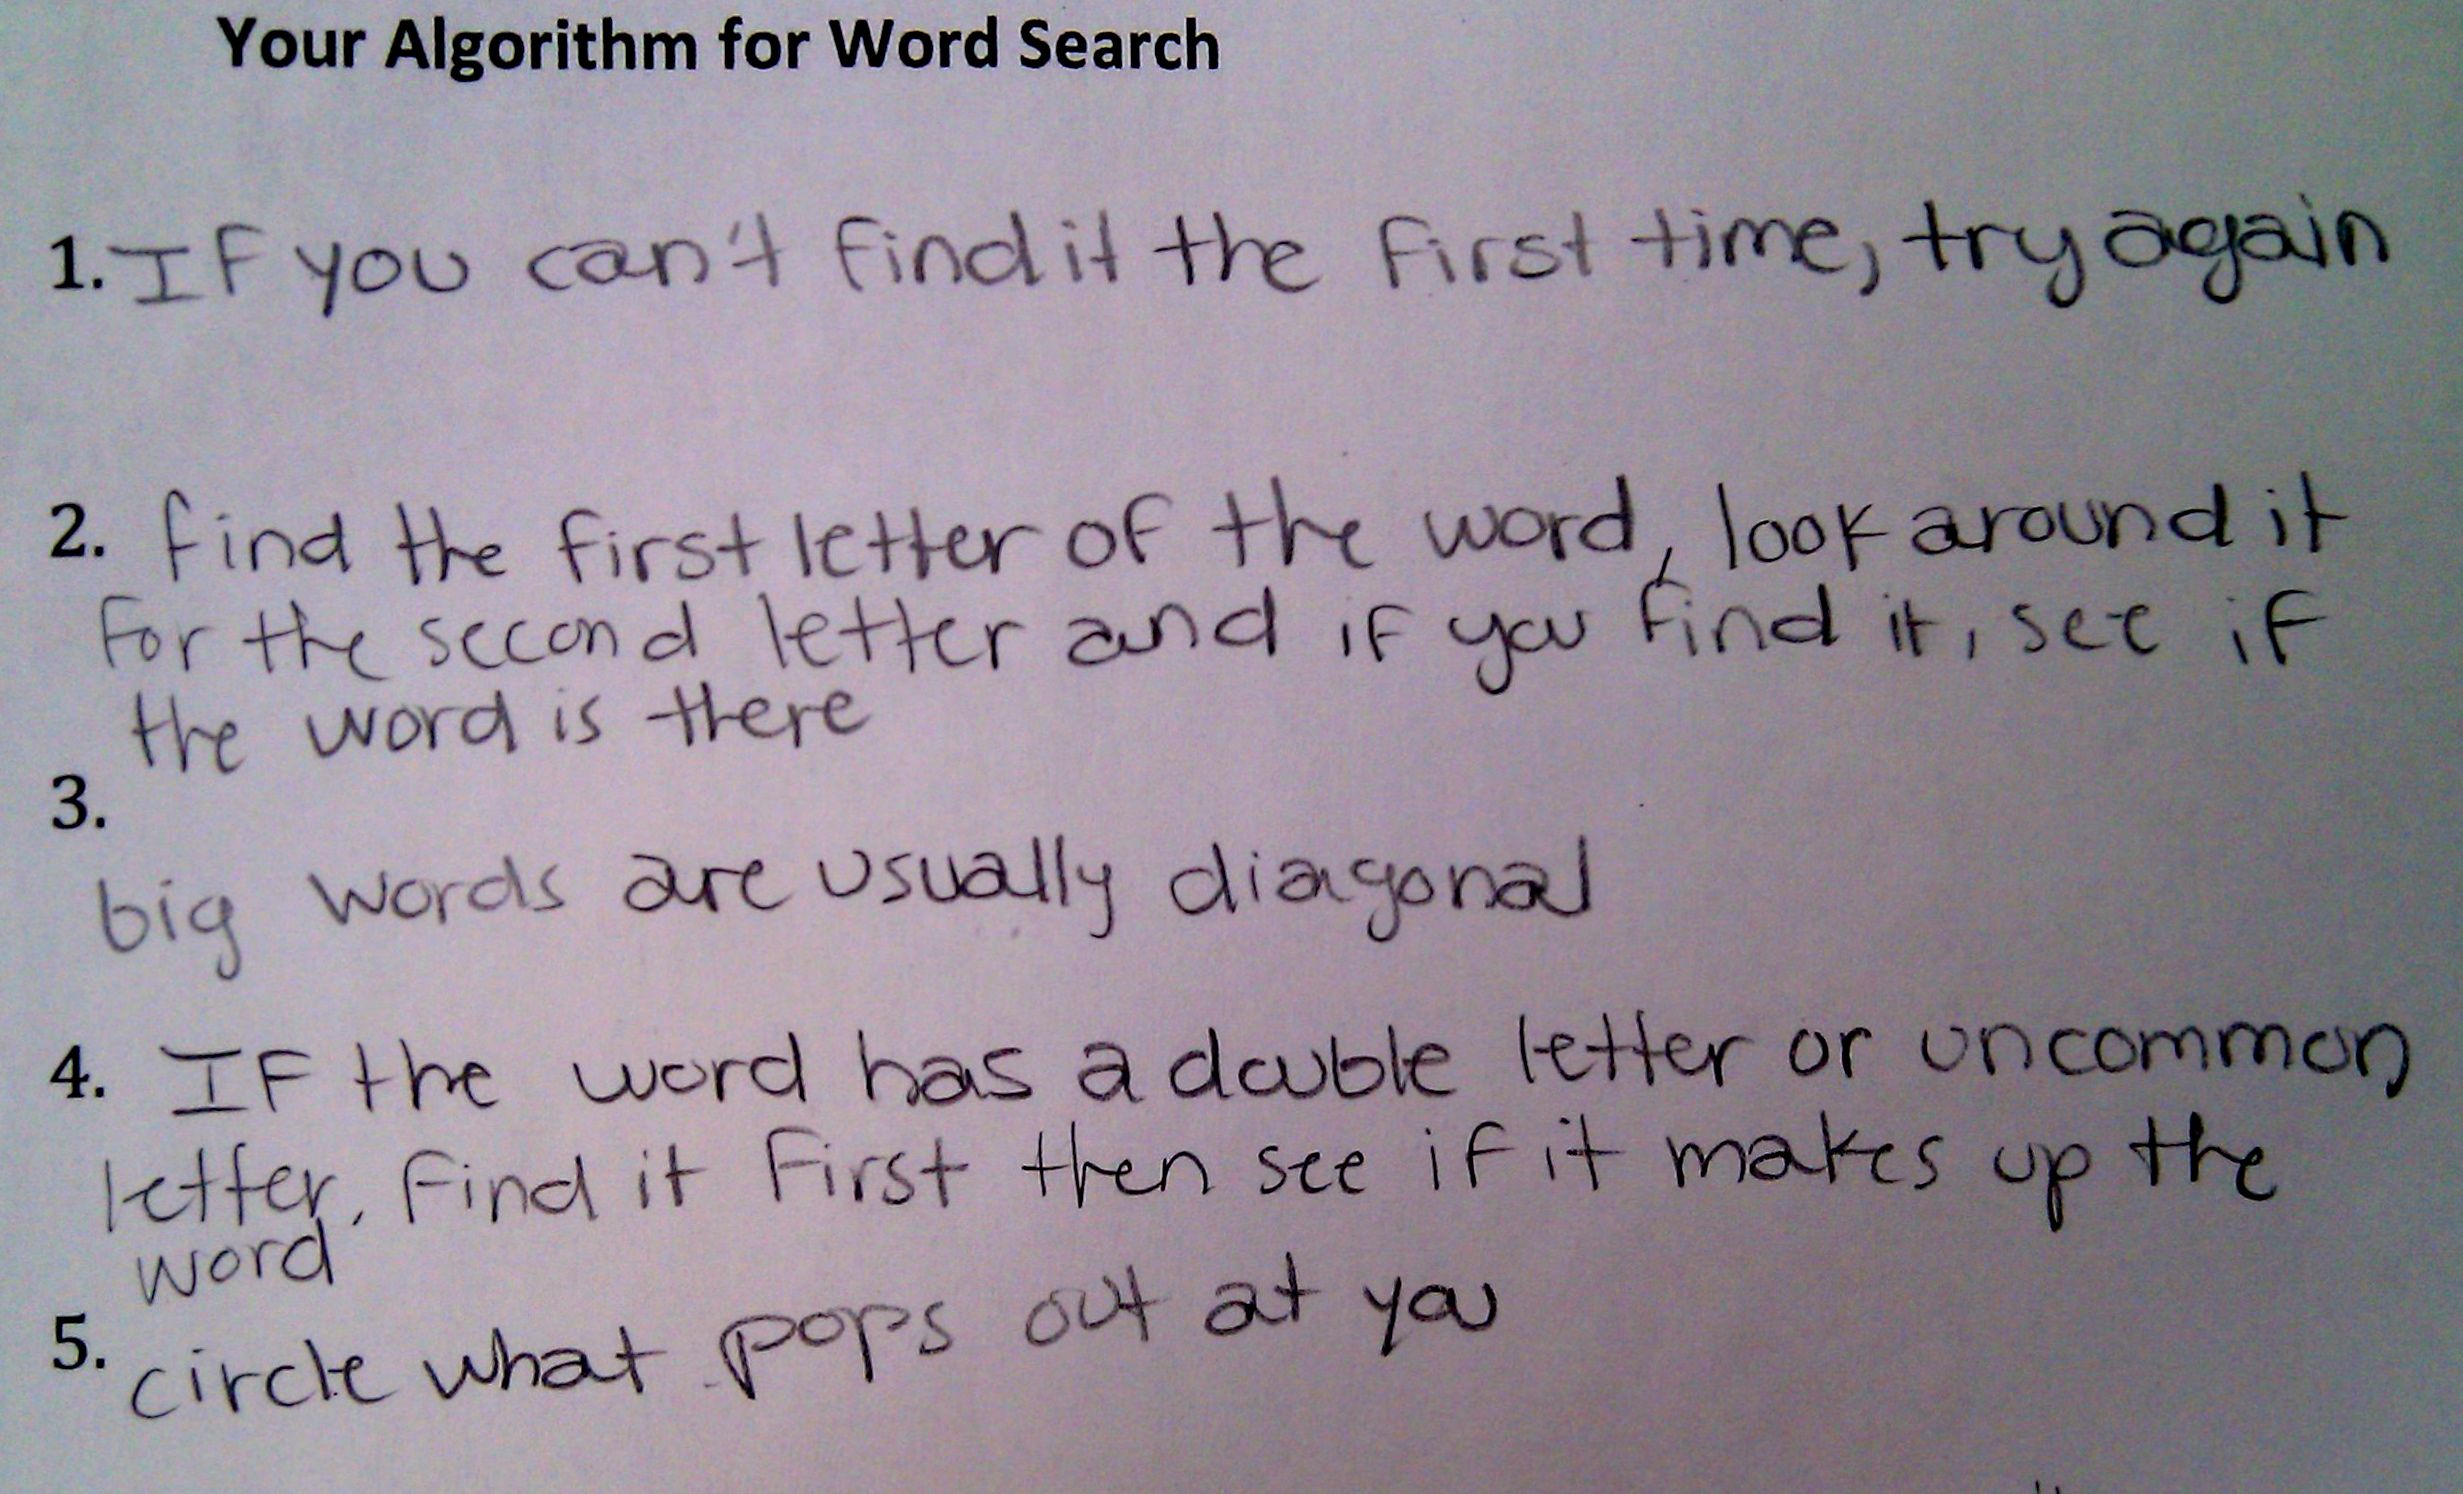
\includegraphics[width=\textwidth]{product/sp-ws-6}
	\caption[Example of a student's algorithm for the Word Search activity.]{Example of a student's algorithm for the Word Search activity. This algorithm uses simple, generalizable instructions.}
	\label{fig:sp-ws-6}
	\end{figure}


%%%%%%%%%%%%%%%%%%%%%%%%%%%%%%%%%%%%%%%%%%%%%%
%%%%%%%%%%%%%%%%%%%%%%%%%%%%%%%%%%%%%%%%%%Elevator
\section{Elevator Control Activity}
	\label{sec:analysis-elevator}

Building on the algorithm writing experience from the word search activity, the elevator control problem is the culmination of the activity sequence. Students built and tested in a simulated environment where the researchers had control of all system mechanics, allowing for only the pertinent interactions to be available. This still allowed for a complex interaction to take place, as the students were were asked to write code to solve an open-ended problem.

\subsection{Expected and Observed Outcomes}

This was the most difficult activity, so it was expected that students would have a hard time gaining traction with the problem. Before a student could be productive, the student would need to understand the constructs of the programming language, begin to comprehend the programming concepts available to them, and form a good understanding of the problem. The most difficult part of this was the latter. The first half of this activity ended up being focused primarily on problem framing. Once students began to comprehend what they were actually trying to do, their productivity improved greatly. Student competence with the programming tools seemed to increase once the problem was understood, indicating that understanding the tool is in part related to having a clear need for it.

\subsection{Problem Framing}
The greatest difficulty in this activity was understanding the task at hand. The setup provided to the students included example code that worked as a fully functional system. The students first questioned what their task was if a working solution was already present. The task was to create an better optimized solution, but what made the example sub-optimal was not apparent.

The example code would go to every floor that was requested in the order that the requests were made. This solution works fine for simple examples where the request queue has a small number of requests, or floors are requested in a convenient order. There are many common examples, however, that illustrate the sub-optimal nature of this system. One such example is if the elevator is on the first floor, and the buttons five, three, and four are quickly pressed, in that order. At the first button press, the elevator will immediately start moving towards the fifth floor. Assume the button presses were complete by the time the elevator reaches the second floor. It now has requests to service the third, fourth, and fifth floors, and is already moving upwards. The example code will skip the people waiting on the third and fourth floors and go straight to the fifth floor. At that point it will skip the fourth floor again as it moves to the third floor, as that was the order that the buttons were pressed. If a person entering on the fifth floor then made a request, that request would not even be considered until all the previously queued pickups had completed.

The above example and ones like it were used by the researchers to help illustrate what was wrong with the example code. The researchers did not explicitly state what was wrong, but guided the students in running such examples and led them to reach their conclusions about inefficiency. Once this inefficiency was understood the students were observed becoming more effective in creating a solution.

%\subsection{Observed Behaviors}
%\subsection{Wrapup Discussion}

\subsection{Elevator Control Results}

\begin{figure}
\centering
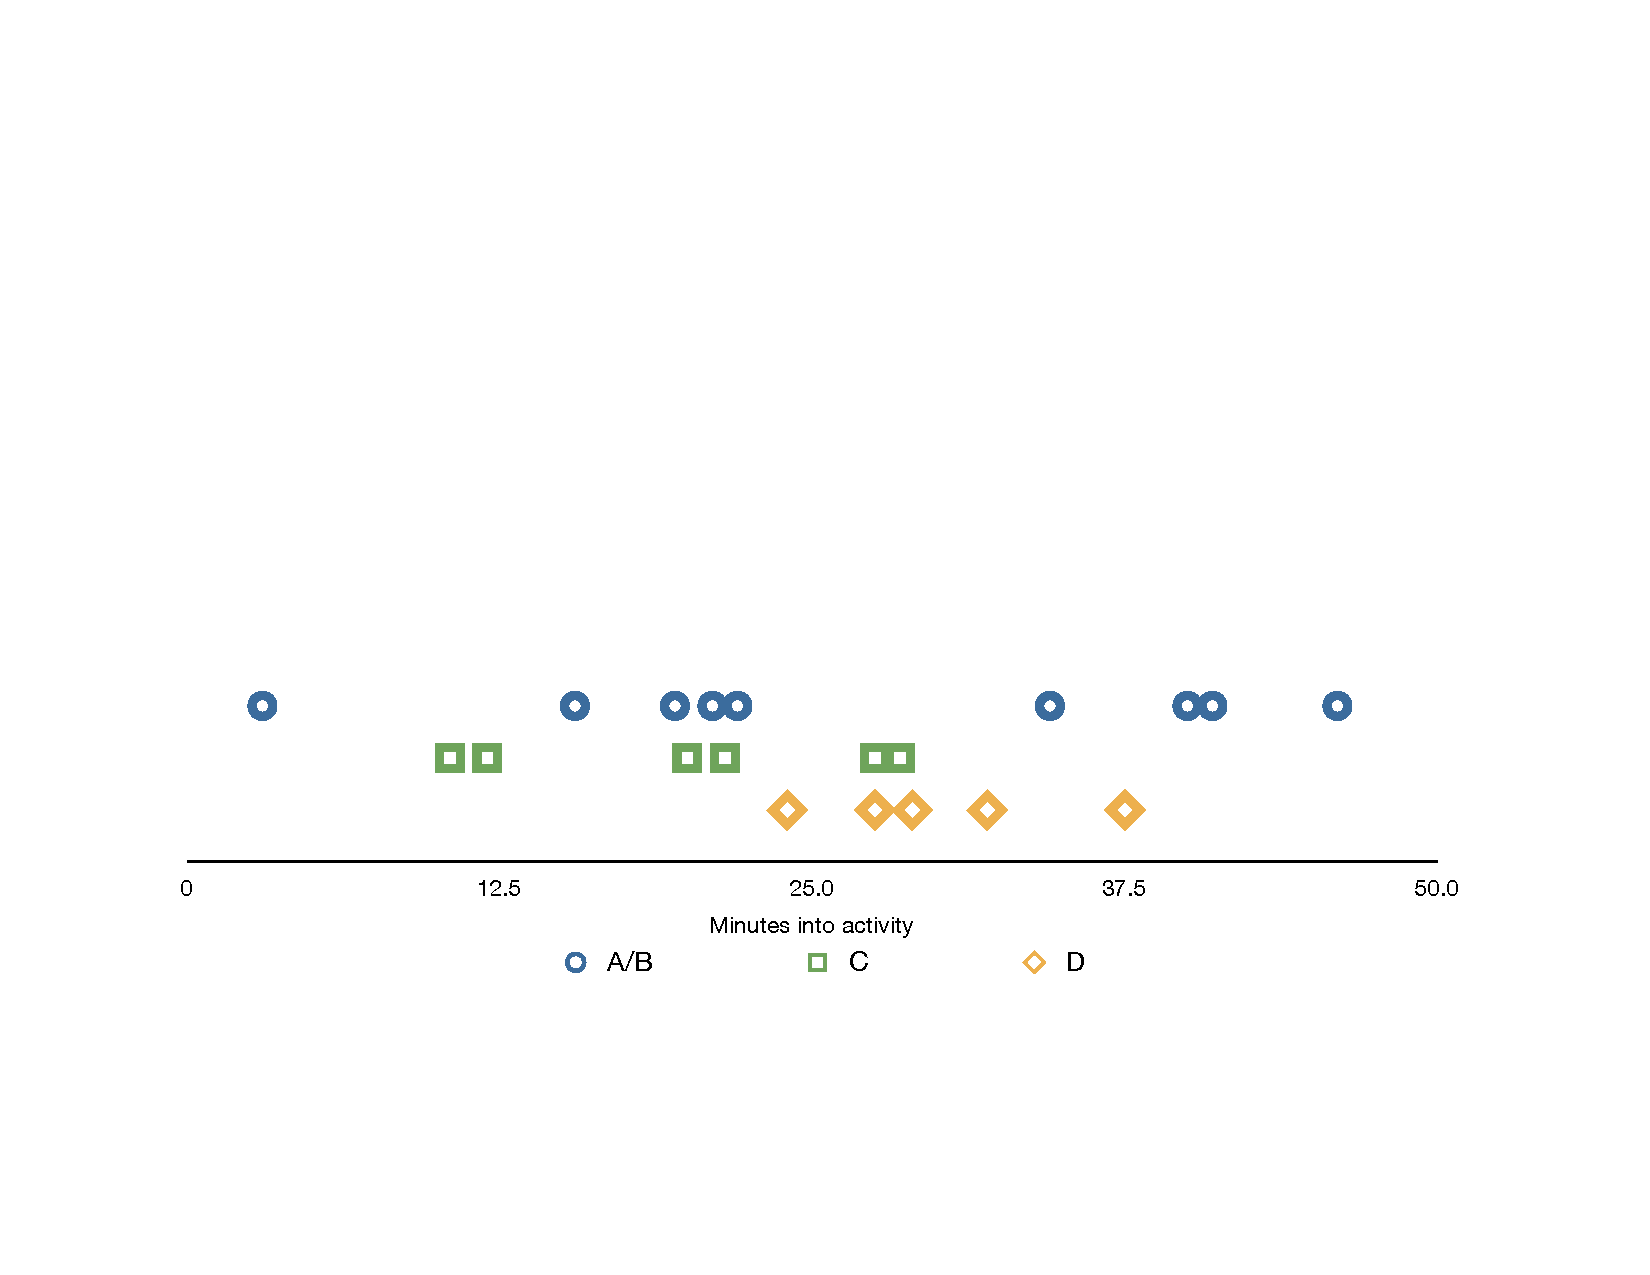
\includegraphics[width=\textwidth]{timelines/elevator-2.pdf} 
\caption[Elevator Control activity iteration timeline.]{Elevator Control activity iteration timeline. Each mark represents a test occurring for the specified students. Each row represents a different student group. The horizontal axis is time, in minutes. All students considered themselves done and stopped working after their final test.}
\label{fig:elevator-timeline}
\end{figure}

Student iteration data is shown in Figure~\ref{fig:elevator-timeline}. The three groups exhibited different amounts of introductory time in this activity, ranging from a short three minutes (group~A/B) to nearly half the session time at 24 minutes (student~D). Each student stopped working after their group's final test, concluding that they had completed the exercise. Student~C reached this point first, followed by student~D and dyad~A/B respectively. 

This activity was included for numerical analysis. The results are shown in Table~\ref{tab:results-elevator}. In this session, success was correlated both with tight iteration and longer introductory time. The two groups who succeeded in both a working solution and generalized process spent at least a third of their total time exploring the problem, and then iterated quickly at regular intervals. The most pronounced correlation is the short introductory time of dyad~A/B, who were the only group not to successfully complete the activity. Only one of the students had any previous experience with the Scratch system. Interestingly, that one student was in the group that did not succeed in this activity.

\begin{table}
\begin{centering}
\begin{tabular}{l c c c}
	\toprule
					& A/B 	& C 		& D 		\\ \midrule
	Iteration Count          & 9 		& 6 		& 5		\\ \midrule
	Time per iteration 	& 5.3 min	& 3.6 min	& 3.4 min 		\\ \midrule
	St.Dev. of time per iteration 	& 4.4 min & 2.9 min & 1.4 min \\ \midrule
	Non-iterating time 	& 7\%      & 36\%	& 64\% 	\\ \midrule
	Success (0,1,2)	& 0		& 2		& 2		\\ 
	\bottomrule
\end{tabular}
\caption[Results from Elevator Control activity.]{Results from Elevator Control activity. The students of dyad~C/D chose to work separately in this session. There are no data for dyad~E/F.}
\label{tab:results-elevator}
\end{centering}
\end{table}

The use of a simulator in Scratch was largely successful. All but one of the students had no prior experience yet were able to piece together functional control programs. Beyond that, students were able, to varying degrees, create programs that did as they intended. In one case a student's goal was modified as the student learned about the capabilities and limitations of the system.